\documentclass[lettersize,journal]{IEEEtran}

\usepackage{amsmath,amsfonts,amssymb}
\usepackage{array}
\usepackage{stfloats}
\usepackage{url}
\usepackage{graphicx}
\usepackage{cite}
\hyphenation{op-tical net-works semi-conduc-tor IEEE-Xplore}
\def\BibTeX{{\rm B\kern-.05em{\sc i\kern-.025em b}\kern-.08em
    T\kern-.1667em\lower.7ex\hbox{E}\kern-.125emX}}

\urlstyle{same}

% Float spacing: IEEEtran defaults leave generous gaps around floats.
% Tightened to recover vertical space without altering figure content.
\setlength{\textfloatsep}{4pt plus 1pt minus 1pt}
\setlength{\floatsep}{6pt plus 2pt minus 2pt}
\setlength{\intextsep}{6pt plus 2pt minus 2pt}
\setlength{\dbltextfloatsep}{4pt plus 1pt minus 1pt}
\setlength{\dblfloatsep}{6pt plus 2pt minus 2pt}
\setlength{\abovecaptionskip}{3pt}
% Float packing: IEEEtran's defaults reserve a large fraction of each
% column for text, which strands whitespace on figure-heavy pages.
% Raising the float fractions lets LaTeX fill those pages properly.
\renewcommand{\topfraction}{0.95}
\renewcommand{\bottomfraction}{0.95}
\renewcommand{\textfraction}{0.05}
\renewcommand{\floatpagefraction}{0.85}
\renewcommand{\dbltopfraction}{0.95}
\renewcommand{\dblfloatpagefraction}{0.85}
\setlength{\belowcaptionskip}{0pt}

\begin{document}

\title{Second-Order Cooperative Field Estimation for
Multirobot Tracking of Coherent Flow Structures}

\author{Christopher Waight and Christopher A. Kitts,~\IEEEmembership{Senior Member,~IEEE}
\thanks{C. Waight is a PhD Candidate in the Robotic Systems Laboratory, Department of Mechanical Engineering, Santa Clara University, Santa Clara, CA 95053 USA (e-mail: cwaight@scu.edu)}
\thanks{C. A. Kitts is Professor and Director of the Robotic Systems Laboratory, Department of Mechanical Engineering, Santa Clara University, Santa Clara, CA 95053 USA (e-mail: ckitts@scu.edu)}
}
\markboth{IEEE Systems Journal}%
{Waight and Kitts: Second-Order Cooperative Field Estimation for Multirobot Tracking of Coherent Flow Structures}

\maketitle

\begin{abstract}
Adaptive navigation is the process of modifying a robot's or a system of robots' motion in
real time based on measurements taken while moving. This paper applies
that process to the boundaries that organize short-term transport in a
flow, the strain-dominated curves across which water masses separate
and along which floating material collects. Existing robotic trackers
of such structures either commit to the structure's identity and pre-straddle it before
tracking begins or accumulate an estimate over a finite integration
horizon. We show that a second-order fit of the local flow removes both
requirements. A cooperative estimator recovers the local quadratic field
model from one synchronous sample, six robots being the minimum for the
unconstrained model. A linear fit gives the velocity gradient at a single
point. The quadratic fit gives it as a field over the formation, so any
quantity built from the velocity gradient comes with its own gradient in
closed form. We build an adaptive navigation primitive on each of two such
quantities, the Jacobian determinant and the smaller rate-of-strain
eigenvalue. Each locates a separating boundary and navigates to and along
it from instantaneous measurements, with no integration horizon and no
pre-straddling. The choice of surrogate sets a tradeoff. Monte Carlo
sweeps show the determinant tracker withstands about four to five times
more measurement noise than the strain tracker, while in a rotating-frame trial only the strain
tracker, which is objective, holds the same material path. On Santa
Barbara Channel radar currents, both primitives follow the same dominant
transport corridor.

\end{abstract}

\begin{IEEEkeywords}
Multirobot Systems, Adaptive Navigation, Coherent Structures,
Okubo-Weiss, Rate of Strain, Objectivity, Cooperative
Estimation, Cluster Space Control
\end{IEEEkeywords}

\section{Introduction}

\IEEEPARstart{M}{ultirobot} systems (MRS) offer redundancy, increased
throughput, and cooperative behaviors a single vehicle cannot produce,
and they now operate across land, sea, air, and space \cite{1}.
 In adaptive
navigation (AN), a vehicle or group of vehicles modifies its direction and path in real time
from measurements taken while moving \cite{2}. A single vehicle must translate to sense a
gradient, which costs time and misleads in a time-varying field,
whereas a cluster samples simultaneously, tolerates vehicle failures,
adapts its size and shape to the spatial frequencies present, and can
fit a local model of the landscape to steer on its features
\cite{2,3,4}.

AN in scalar fields is well developed. Each
robot contributes one scalar measurement to a policy that reaches and
follows a feature, and formations are sized so that differential
measurements across the cluster recover the gradient and curvature that
policy consumes \cite{4,5}. \"{O}gren, Fiorelli, and Leonard
established cooperative gradient climbing with a formation of mobile
sensors \cite{5}. Bri\~{n}\'{o}n-Arranz, Renzaglia, and Schenato
extended it to the Hessian, five robots on a ring plus one at the
center recovering both in closed form \cite{4}. Kitts, McDonald, and
Neumann developed primitives for extrema finding, contour following,
ridge/trench following, and saddle point station keeping \cite{2}, and
verified ridge, trench, saddle, and front tracking experimentally on an
indoor testbed \cite{3,6}.

Some environments are better modeled as vector fields, which contain features without scalar field equivalents. Critical points, such as sinks, sources, and spewing vortices can be used to model convergence zones and
subsurface leaks \cite{7}.  In \cite{8} a three-robot cluster
estimated the location and type of one from a linear fit of
simultaneous local velocity measurements and used this estimate to adaptively navigate towards and around them. 

Beyond critical points, vector fields have curves that are useful for navigation. For example, dynamic ocean flows contain naturally occurring boundaries known as coherent structures that influence where floating materials like debris and larvae will accumulate or separate \cite{9,10}. Mapping these exact curves allows teams to strategically deploy resources in highly targeted search areas \cite{11,12,13}. Without adaptive navigation, a large scale team must sample a much larger basin to determine where these structures lie.

Coherent structures are typically identified through two primary methods. The first relies on Lagrangian coherent structures (LCS) \cite{14}, typically computed as ridges in the finite-time Lyapunov exponent field \cite{15}, with ongoing research addressing the Lagrangian/Eulerian tradeoff and sparse-trajectory gradient recovery \cite{16,17,18,19,20}. The second method uses instantaneous Eulerian criteria, such as the Okubo-Weiss parameter, to partition flows based solely on the local velocity gradient \cite{21,22}. This instantaneous approach has been generalized to three dimensions \cite{23}, refined for oceanographic use \cite{24}, and applied at scale in mesoscale eddy censuses \cite{25}. However, both of these methods characterize these structures offline using a reconstructed field, which is not well suited to real-time adaptive navigation of a field that evolves in time.  

New work is being done on using AN techniques with MRS in these scenarios. Michini et al. bracket a presumed stable or
unstable manifold with three robots using only local velocity
measurements \cite{26}, an approach inspired by the PIM triple
procedure, extended to $N$ robots \cite{27} and validated
experimentally in gyre-like flows \cite{28,29}. The robots begin on the
manifold and are advected by the flow, and the manifold's identity is
supplied in advance. The saddle point is treated by neither the
controller nor its analysis, and that work reports veering away from
the structure near a saddle in both flow-tank and ocean trials. Kularatne and Hsieh do not presume stable or unstable, but rather, they compute the local FTLE field on board, recovering
type at the cost of a nonzero integration horizon \cite{30}. In both cases, the robotic formation pre-straddles the structure, and does not acquire a structure it does not already occupy.

This paper shows that a second-order fit of the local flow is enough to
acquire and track such a structure from instantaneous measurements. A
linear fit, as in \cite{8}, gives the velocity gradient at one point. A
second-order fit gives it as a field over the formation, so any quantity
built from it comes with its own gradient in closed form. The contributions are
\begin{itemize}
\item a cooperative estimator that recovers the local quadratic model of
a two-component field from one synchronous sample of six robots, the
minimum for the unconstrained model, and that fails only when the robots
lie on a common conic;
\item two surrogates read in closed form from that fit, the
velocity-gradient determinant $D$ and the smaller strain eigenvalue
$s_1$, with the noise behavior of each characterized;
\item two AN primitives, the $D$ tracker and the $s_1$ tracker, that
navigate to the structure and ride along it without pre-straddling;
\item a tradeoff between them, in which the $D$ tracker tolerates more
measurement noise while the $s_1$ tracker, being objective, holds its
path under a rotating observer, which matters for a cluster that cannot
certify its heading.
\end{itemize}

Both primitives run on a simulated double gyre and on measured Santa
Barbara Channel radar currents.

\section{Second-Order Field Estimation}

\subsection{Local Vector Field Polynomials}

A planar vector field assigns a velocity $\mathbf{v}(\mathbf{p}) =
(u(\mathbf{p}), v(\mathbf{p}))$ to each position in space $\mathbf{p} = (x, y)$.
The critical point estimator of \cite{8} fits a plane of each
component of the vector field and solves for the point where $\mathbf{v} = \mathbf{0}$. 

In this work, we extend the linear approximation to the second-order Taylor expansion about the
centroid, $\mathbf{p}_c$. Coordinates are measured
from the centroid throughout this section, so $\mathbf{p}_c = \mathbf{0}$.
\begin{align}
    u(\mathbf{p}) &= a_1 + a_2 x + a_3 y
        \nonumber \\
        &\quad + a_4 xy + \tfrac{1}{2} a_5 x^2 + \tfrac{1}{2} a_6 y^2
        + \mathcal{O}(\|\mathbf{p}\|^3),
        \label{eq:quad_model_u} \\
    v(\mathbf{p}) &= b_1 + b_2 x + b_3 y
        \nonumber \\
        &\quad + b_4 xy + \tfrac{1}{2} b_5 x^2 + \tfrac{1}{2} b_6 y^2
        + \mathcal{O}(\|\mathbf{p}\|^3).
        \label{eq:quad_model_v}
\end{align}

The twelve coefficients of this quadratic model are constants and each is a derivative of the field at
the centroid. The one-half factors cancel the factor of 2 during differentiation.
This gives $a_1 = u(\mathbf{p}_c)$, $a_2 = \partial u/\partial
x|_{\mathbf{p}_c}$, $a_4 = \partial^2 u/\partial x \partial
y|_{\mathbf{p}_c}$, $a_5 = \partial^2 u/\partial x^2|_{\mathbf{p}_c}$,
and likewise for $b_1, \ldots, b_6$ with $v$ in place of $u$.

To estimate these coefficients with robot positions $\mathbf{p}_i = (x_i,
y_i)$, we define the quadratic basis vector
\begin{equation}
    \boldsymbol{\phi}(\mathbf{p}) =
    \bigl[\,1, \; x, \; y, \; xy, \;
    \tfrac{1}{2}x^2, \; \tfrac{1}{2}y^2\,\bigr]^\top,
\end{equation}
whose entries are the terms of
(\ref{eq:quad_model_u})--(\ref{eq:quad_model_v}) in order, so
the recovered coefficients, which we mark with a hat, estimate the Taylor derivatives directly with
no rescaling. Stacking the six basis vectors row-wise gives
the $6 \times 6$ formation matrix $\boldsymbol{\Phi}$, and the coefficient
estimates $\hat{\boldsymbol{\theta}}_u = [\hat{a}_1, \ldots,
\hat{a}_6]^\top$ and $\hat{\boldsymbol{\theta}}_v = [\hat{b}_1, \ldots,
\hat{b}_6]^\top$ solve
\begin{equation}
    \boldsymbol{\Phi}\,\hat{\boldsymbol{\theta}}_u = \mathbf{m}_u, \qquad
    \boldsymbol{\Phi}\,\hat{\boldsymbol{\theta}}_v = \mathbf{m}_v,
    \label{eq:solve}
\end{equation}
where $\mathbf{m}_u = [u_1, \ldots, u_6]^\top$ and
$\mathbf{m}_v = [v_1, \ldots, v_6]^\top$ collect the measurements, $u_i$
and $v_i$ being the field components sampled by robot $i$. 

\subsection{Minimality}
\label{sec:minimality}

Six robots is the minimum for recovery of the unconstrained local
quadratic model of a two-component planar field from one synchronous
sample. Each robot contributes one equation per component to
(\ref{eq:solve}), and each system has six unknowns, so fewer than six
robots leave the solution set a positive-dimensional affine subspace.

Any method for approximating the quadratic field using five equations or
fewer is not providing a unique solution, but a family of solutions.
Alternately, the technique is using a structural prior, such as assuming
divergence-free flow by imposing $\operatorname{tr}(\mathbf{J}) = 0$, where
$\mathbf{J} = \nabla\mathbf{v}$ is the velocity gradient tensor, whose
centroid entries are the first-order coefficients $a_2$, $a_3$, $b_2$,
$b_3$. We do not impose any priors on the field, as horizontal surface
currents are not divergence free, so imposing
$\operatorname{tr}(\mathbf{J}) = 0$ would bias every recovered coefficient.

For this study, we chose the pentagon-plus-center formation and use it
throughout. It is the smallest uniform ring plus center on which \cite{4}
recovers a scalar Hessian exactly for quadratic signals, independent of
the formation's orientation. The same symmetry makes the noise gains of
the fit here independent of formation heading.

However, any formation of six or more robots suffices provided
$\boldsymbol{\Phi}$ is nonsingular. This nonsingularity fails exactly
when the robots lie on a common conic. For example, a standard ring
formation is degenerate at any size, since the ring itself is the
conic.


\subsection{Estimator Sensitivity}
\label{sec:sensitivity}

The accuracy of the estimator is affected by the formation of the
robots, the noise on each robot's measurements, and the error in each
robot's position.

\subsubsection{Formation}
The rank of the formation matrix $\boldsymbol{\Phi}$ determines whether
a unique fit exists, and its condition number $\kappa(\boldsymbol{\Phi})$
indicates how much the fit amplifies noise. Condition numbers are
reported on the radius-normalized $\boldsymbol{\Phi}$, with each column
of order $q$ divided by $\rho^{\,q}$. Without this normalization, the
quadratic columns shrink as $\rho^{2}$ and a healthy formation would
appear degenerate. The normalized matrix depends only on the formation's
shape, and the pentagon-plus-center formation gives
$\kappa(\boldsymbol{\Phi}) = 8.26$ at every radius. The size of the formation instead scales the noise on each
coefficient by $\rho^{-q}$, so a larger formation suppresses noise most
in the second-order terms. The condition number grows as the robots
drift toward a common conic. For example, moving the center robot out
to $0.99\rho$ places all six robots within $0.6\%$ of a common circle
and raises $\kappa(\boldsymbol{\Phi})$ to $564$. The fit degrades
continuously on the way to the degeneracy of
Section~\ref{sec:minimality}, with no threshold at which it fails.

\subsubsection{Measurement Noise}
Each robot carries its own sensor, so the measurement noise of one robot
is independent of the others. Furthermore, the estimator uses only
instantaneous readings, so each cycle's fit sees only that cycle's
noise. The noise is modeled as additive on each reading,
\begin{equation}
    u_i^m = u(\mathbf{p}_i) + \eta_i^u, \qquad
    v_i^m = v(\mathbf{p}_i) + \eta_i^v,
    \label{eq:meas_noise}
\end{equation}
with $\eta \sim \mathcal{N}(0, \sigma_{uv}^2)$. The fit is linear in the
measurements, so the noise reaches the coefficients as
$\boldsymbol{\Phi}^{-1}\boldsymbol{\eta}^u$ and
$\boldsymbol{\Phi}^{-1}\boldsymbol{\eta}^v$, where $\boldsymbol{\eta}^u$
and $\boldsymbol{\eta}^v$ stack the noise of the six robots. Both are
zero-mean, so the coefficient estimates are unbiased.

\subsubsection{Position Noise}
A robot with position error
$\boldsymbol{\xi}_i \sim \mathcal{N}(\mathbf{0}, \sigma_p^2\mathbf{I})$
samples the field at $\mathbf{p}_i + \boldsymbol{\xi}_i$, but the fit is
built from its nominal position $\mathbf{p}_i$. The formation matrix is
therefore wrong by $\Delta\boldsymbol{\Phi}$, whose row $i$ is
$\boldsymbol{\phi}(\mathbf{p}_i + \boldsymbol{\xi}_i)^{\top} -
\boldsymbol{\phi}(\mathbf{p}_i)^{\top}$. Under the quadratic model the
measurements are
$\mathbf{m}_u = (\boldsymbol{\Phi} + \Delta\boldsymbol{\Phi})
\boldsymbol{\theta}_u$, and the fit returns
\begin{equation}
    \hat{\boldsymbol{\theta}}_u = \boldsymbol{\theta}_u
        + \boldsymbol{\Phi}^{-1}\Delta\boldsymbol{\Phi}\,
          \boldsymbol{\theta}_u ,
    \label{eq:pos_noise}
\end{equation}
and likewise for $\hat{\boldsymbol{\theta}}_v$. To first order, entry
$i$ of $\Delta\boldsymbol{\Phi}\,\boldsymbol{\theta}_u$ is
$\nabla u \cdot \boldsymbol{\xi}_i$, the change in $u$ across the
displacement. This error vanishes in uniform flow and grows with the
local gradient, so unlike measurement noise it depends on the field.
Its variance is $\lVert\nabla u\rVert^2\sigma_p^2$ for $u$ and
$\lVert\nabla v\rVert^2\sigma_p^2$ for $v$, and the two average to
$\tfrac{1}{2}\lVert\mathbf{J}\rVert_F^2\sigma_p^2$. Combining both noise
sources gives one effective noise level
\begin{equation}
    \sigma_{\mathrm{eff}}^2 = \sigma_{uv}^2
        + \tfrac{1}{2}\lVert\mathbf{J}\rVert_F^2\,\sigma_p^2 ,
    \label{eq:sigma_eff}
\end{equation}
which is exact only when the two gradients have equal norm.
Additionally, the same $\Delta\boldsymbol{\Phi}$ corrupts both fits, so
the $u$ and $v$ errors at one robot are correlated, with correlation
coefficient
$\nabla u \cdot \nabla v / (\lVert\nabla u\rVert\,\lVert\nabla v\rVert)$.


% ###### I have proofread everything above this line ######

\subsection{Eulerian Surrogates}
\label{sec:surrogates}

Lagrangian methods locate coherent structures by integrating particle
trajectories over a finite time window \cite{14,15}. This paper instead
reads them from the instantaneous geometry of the velocity field, which
the six-robot fit already provides. Two fields computed from that fit
mark the separatrix. The first is the determinant of the velocity
gradient, and the second is the smaller eigenvalue of its symmetric
part.

\subsubsection{Determinant Field}
The fitted coefficients define the velocity gradient at every point of
the footprint. Differentiating the quadratic model gives a Jacobian whose
entries are affine in position,
\begin{equation}
    \hat{\mathbf{J}}(\mathbf{p}) =
    \begin{bmatrix}
        \hat{a}_2 + \hat{a}_5 x + \hat{a}_4 y &
        \hat{a}_3 + \hat{a}_4 x + \hat{a}_6 y \\
        \hat{b}_2 + \hat{b}_5 x + \hat{b}_4 y &
        \hat{b}_3 + \hat{b}_4 x + \hat{b}_6 y
    \end{bmatrix}.
    \label{eq:Jhat}
\end{equation}
The determinant $\hat{D}(\mathbf{p}) = \det\hat{\mathbf{J}}(\mathbf{p})$
is therefore exactly quadratic over the footprint. Its value, gradient,
and Hessian at the centroid are polynomials in the coefficients. The
value is $\hat{D}_0 = \hat{a}_2\hat{b}_3 - \hat{a}_3\hat{b}_2$, and the
Hessian is
\begin{equation}
    \hat{\mathbf{H}}_{D,0} =
    \begin{bmatrix}
        2(\hat{a}_5\hat{b}_4 - \hat{a}_4\hat{b}_5) &
        \hat{a}_5\hat{b}_6 - \hat{a}_6\hat{b}_5 \\
        \hat{a}_5\hat{b}_6 - \hat{a}_6\hat{b}_5 &
        2(\hat{a}_4\hat{b}_6 - \hat{a}_6\hat{b}_4)
    \end{bmatrix},
    \label{eq:hess_det}
\end{equation}
which is constant over the footprint.

For incompressible flow the determinant is a negative multiple of the
Okubo-Weiss parameter \cite{21,22}, so the two carry the same partition of
the flow. Where $D < 0$ the flow is strain-dominated, and where $D > 0$
it is rotation-dominated. Separatrices run along the trenches of $D$
inside the strain-dominated regions.

Every term of $\hat{D}$, its gradient, and its Hessian comes in an
opposite-sign pair such as $\hat{a}_2\hat{b}_3 - \hat{a}_3\hat{b}_2$.
The robots are independent and both fits share
$\boldsymbol{\Phi}^{-1}$, so a correlation between the $\hat{a}$ and
$\hat{b}$ errors inflates both products of a pair equally, and the
subtraction cancels it. The $D$ estimates are therefore unbiased under
measurement noise, and under position noise to first order.

\subsubsection{Strain Eigenvalue Field}
The same fitted Jacobian carries the second field through its symmetric
part, the rate-of-strain tensor
$\hat{\mathbf{S}} = \tfrac{1}{2}(\hat{\mathbf{J}} + \hat{\mathbf{J}}^{\top})$.
At the centroid its mean, deviatoric normal, and shear strain are
$\hat{\mu} = (\hat{a}_2 + \hat{b}_3)/2$,
$\hat{s}_n = (\hat{a}_2 - \hat{b}_3)/2$, and
$\hat{s}_s = (\hat{a}_3 + \hat{b}_2)/2$, and each is affine in position.
The eigenvalues of $\hat{\mathbf{S}}$ are
$\hat{s}_{1,2} = \hat{\mu} \mp \hat{r}$ with
$\hat{r} = \sqrt{\hat{s}_n^2 + \hat{s}_s^2}$. Their eigenvectors
$\mathbf{e}_1$ and $\mathbf{e}_2$ are the compression and stretching
directions. The gradient of the smaller eigenvalue follows by the chain
rule,
\begin{equation}
    \nabla\hat{s}_1 = \nabla\hat{\mu}
        - \frac{\hat{s}_n\nabla\hat{s}_n + \hat{s}_s\nabla\hat{s}_s}{\hat{r}},
    \label{eq:grad_s1}
\end{equation}
with $\nabla\hat{\mu}$, $\nabla\hat{s}_n$, and $\nabla\hat{s}_s$ read
from the second-order coefficients. Unlike $\hat{D}$, $\hat{s}_1$ has no
usable Hessian. It is an affine function minus the norm of an affine
map, so it is concave over the footprint for every field and formation.

Serra and Haller define objective Eulerian coherent structures (OECS)
from these eigenvalues and eigenvectors \cite{17}. An attracting OECS is a
trench of $s_1$ tangent to $\mathbf{e}_2$, and floating material has been
observed at sea to collect onto such curves \cite{10}. A repelling OECS is a
ridge of $s_2$ tangent to $\mathbf{e}_1$, along which neighboring
material separates. In incompressible flow $s_2 = -s_1$, so repelling
structures are also trenches of $s_1$, and one tracker rides both.

Recovering $\hat{s}_1$ requires a norm, which biases it under either
noise channel. The error $\boldsymbol{\epsilon}$ in
$(\hat{s}_n, \hat{s}_s)$ is zero-mean, but its component transverse to
the true $(s_n, s_s)$ always lengthens the norm. Expanding to second
order in $\boldsymbol{\epsilon}$ gives
\begin{equation}
    E[\hat{s}_1] - s_1 \approx -\frac{\sigma_r^2}{2r},
    \label{eq:s1_bias}
\end{equation}
where $r$ is the true deviatoric strain magnitude and $\sigma_r$ is the
standard deviation of each strain component. The approximation holds
while $\sigma_r$ is small against $r$. The bias is always negative, so
$\hat{s}_1$ reads a trench deeper than it is.

\subsubsection{Relation Between the Fields}
Both fields are read from the same fitted Jacobian, so moving between
them changes nothing in the estimator. Where the vorticity
$\omega = \partial v/\partial x - \partial u/\partial y$ vanishes,
$\mathbf{J}$ equals $\mathbf{S}$ and $D = s_1 s_2$, which is $-s_1^2$ in
incompressible flow. Along such a curve the two fields share their
trenches. Elsewhere the spin $\mathbf{W} = \mathbf{J} - \mathbf{S}$, the
antisymmetric part of $\mathbf{J}$ that carries the vorticity, separates
them. It also separates them across observers. A frame rotating at rate
$\Omega$, with rotation $\mathbf{Q}$, adds a uniform spin that raises
$\omega$ to $\omega + 2\Omega$. The strain tensor only co-rotates, so
$s_1$ is objective \cite{17}, while the determinant keeps the spin,
\begin{equation}
    D' = D + \Omega\,\omega + \Omega^2 .
    \label{eq:D_not_objective}
\end{equation}
Relatively rotating observers therefore disagree about where the
trenches of $D$ lie. In general neither instantaneous field is
guaranteed to mark the material transport structure \cite{16}.

\subsection{The Double-Gyre Example}
\label{sec:dg_example}

The double gyre is
a benchmark flow on which both fields mark the material transport structure
exactly, and every
quantity of interest has a closed form. The flow is two counter-rotating gyres in a
closed basin, separated by a separatrix that runs between two saddle points on
the basin walls. We use the steady member of the Shadden
family~\cite{15}, shifted from the canonical domain
$[0,2]\times[0,1]$ to $[-1,1]\times[-0.5,0.5]$ to center it on the origin. The
shift is $x_f = x + 1$, $y_f = y + 0.5$, where $(x_f, y_f)$ are field-frame and
$(x, y)$ world-frame coordinates. Both are non-dimensional throughout the
double-gyre experiments. The field is
\begin{equation}
u = -\pi A \sin(\pi x_f)\cos(\pi y_f), \quad
v = \pi A \cos(\pi x_f)\sin(\pi y_f),
\label{eq:dg_u}
\end{equation}
with $A = 0.1$. The separatrix is the line $x = 0$, the saddle points are
$\mathbf{p}_1^* = (0, -0.5)$ and $\mathbf{p}_2^* = (0, 0.5)$, and the gyre
centers are $(\pm 0.5, 0)$.

The benchmark quantities follow from the Jacobian of the field. Where
a partial derivative of the true field is meant rather than a fitted
coefficient, it is written in subscript form, $u_x$, $u_{xy}$, and so on. The
Jacobian entries are
$u_x = -\pi^2 A \cos\pi x_f \cos\pi y_f = -v_y$ and
$u_y = \pi^2 A \sin\pi x_f \sin\pi y_f = -v_x$. The flow is therefore
incompressible, and its determinant and Hessian are
\begin{equation}
\begin{aligned}
D(\mathbf{p}) &= -\tfrac{1}{2}\pi^4 A^2 \left(\cos 2\pi x_f + \cos 2\pi y_f\right),\\
\mathbf{H}_D &= 2\pi^6 A^2
\begin{bmatrix} \cos 2\pi x_f & 0 \\ 0 & \cos 2\pi y_f \end{bmatrix}.
\end{aligned}
\label{eq:det_analytic_main}
\end{equation}
The Hessian is diagonal everywhere, so its eigenvectors lie on the coordinate
axes.

The landscape of $D$ is a grid of trenches around rotation-dominated gyres,
each inside an Okubo-Weiss diamond $x_f \pm y_f \in \tfrac{1}{2} + \mathbb{Z}$
where $D > 0$. The trenches lie on the lines $x \in \{-1, 0, 1\}$ and
$y = \pm 0.5$, the separatrix and the four basin walls, which cross at right
angles at $\mathbf{p}_1^*$, $\mathbf{p}_2^*$, and the four domain corners.

Along the separatrix $D = -\pi^4 A^2 \sin^2 \pi y$. The trench is deepest at
the two saddles and rises to a crest, $D = 0$, at the origin
(Fig.~\ref{fig:trench_cross}). The crest divides the separatrix into an upper
and a lower segment. On $x = 0$ the Hessian reduces to
$\mathbf{H}_D = 2\pi^6 A^2\,\mathrm{diag}(1, -\cos 2\pi y)$.
The transverse curvature $2\pi^6 A^2$ is the same along the whole separatrix.
The along-trench curvature is negative for $|y| < 0.25$ and positive beyond, so
each segment is concave along its length on its inner half and convex on its
outer half. At a saddle both curvatures are positive, and $D$ has a local
minimum where the separatrix crosses the wall.

The vorticity ties the $s_1$ field to the $D$ field on this flow. It is
$\omega = -2\pi^2 A \sin\pi x_f \sin\pi y_f$, which vanishes where $x_f$ or
$y_f$ is an integer, exactly on the trench grid of $D$. There
$\mathbf{J} = \mathbf{S}$ and $D = -s_1^2$ (Section~\ref{sec:surrogates}), so
the two fields share every trench. The shear strain vanishes identically, so
$\mathbf{S} = \mathrm{diag}(u_x, -u_x)$ everywhere. This gives
\begin{equation}
s_1 = -\pi^2 A \left|\cos\pi x_f \cos\pi y_f\right|,
\label{eq:s1_analytic_main}
\end{equation}
with minima $s_1 = -\pi^2 A$ where the grid lines cross, at $\mathbf{p}_1^*$,
$\mathbf{p}_2^*$, and the four domain corners. The eigenvectors of
$\mathbf{S}$ lie on the coordinate axes except on the lines $x = \pm 0.5$ and
$y = 0$ through the gyre centers, where $u_x = 0$, $\mathbf{S}$ vanishes, and
both eigenvectors are undefined. The line $y = 0$ crosses the separatrix at
the origin, an isotropic point of $\mathbf{S}$ at the crest of $D$.

On the upper segment $u_x < 0$, so the stretching
eigenvector $\mathbf{e}_2$ is tangent to the trench. On the lower segment
$u_x > 0$, and the compression eigenvector $\mathbf{e}_1$ is tangent. By the
OECS definition of Section~\ref{sec:surrogates}, the upper segment is an
attracting OECS and the lower a repelling OECS. The two meet at the isotropic
point, where the tangent swaps between eigenvectors (Fig.~\ref{fig:s1_trench}).

\begin{figure}[!tb]
    \centering
    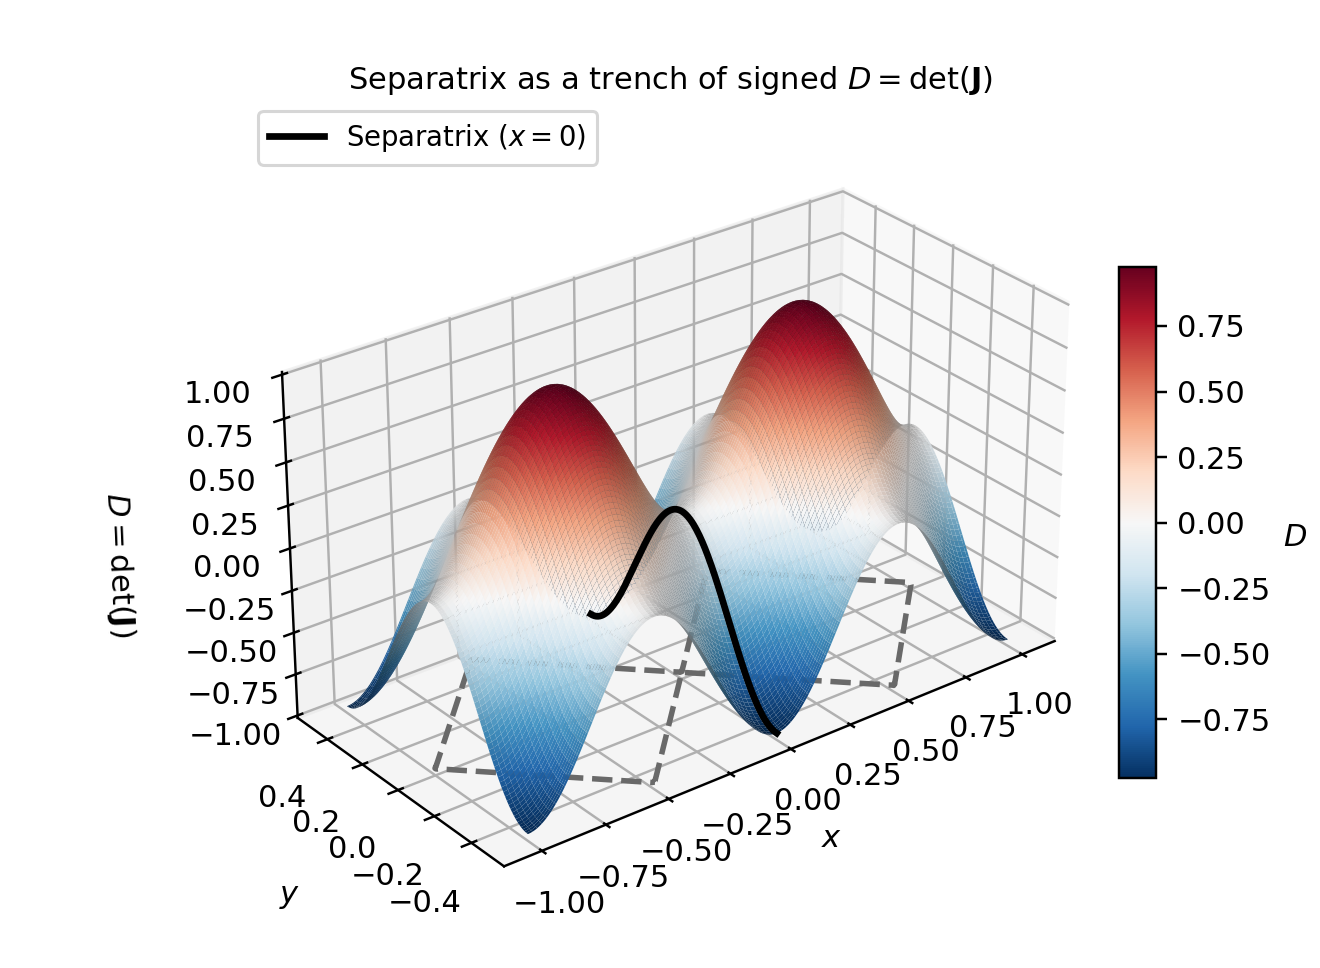
\includegraphics[width=0.30\textwidth]{figures/detJ_trench_cross_section.png}
    \caption{Signed $D$ as an elevation surface over the double gyre.
    The gyre centers rise as peaks ($D > 0$). The separatrix at $x = 0$
    (bold) is a trench of $D$, deepest at the saddles and rising to
    $D = 0$ at the origin.}
    \label{fig:trench_cross}
\end{figure}

\begin{figure}[!tb]
    \centering
    \includegraphics[width=0.30\textwidth]{figures/s1_trench_surface.png}
    \caption{$s_1$ as an elevation surface over the same domain as
    Fig.~\ref{fig:trench_cross}. The separatrix at $x = 0$ is a trench on
    both segments, deepest at the saddles. The trench tangent is
    $\mathbf{e}_2$ on the upper, attracting segment and $\mathbf{e}_1$ on
    the lower, repelling segment. The two swap at the isotropic point of
    $\mathbf{S}$ at the origin, where the $D$ crest of
    Fig.~\ref{fig:trench_cross} sits.}
    \label{fig:s1_trench}
\end{figure}

\section{Control Architecture}
\label{sec:controllers}

\subsection{Three-Layer Structure}
\label{sec:arch}

The control architecture is the established multilayer approach of prior
cluster space adaptive navigation studies \cite{8,32}, shown in
Fig.~\ref{fig:control_architecture}. There are three layers: (1) an
adaptive navigation layer that estimates the local field and generates the
cluster velocity command, (2) a cluster controller layer that maintains
the formation and translates between cluster space and robot space
variables, and (3) a robot controller layer that converts each robot's
velocity command into actuation. Field samples enter only at the adaptive
navigation layer. The layers below it operate on velocity commands and
positions alone.

The adaptive navigation layer has three functional blocks. The feature
estimation block fits the local quadratic model (\ref{eq:solve}) to the
six field samples and robot positions. The navigation controller evaluates
the active primitive, including its mode logic, and emits a desired
centroid velocity $\dot{\mathbf{p}}_c$. Each channel of that command
saturates through $c_{\max}\tanh(c/c_{\max})$ and is scaled by a fixed
navigation gain $k$, so the commanded centroid speed never exceeds
$\sqrt{2}\,k\,c_{\max}$. The formation controller regulates the cluster
shape to the desired shape parameters by proportional feedback. The two
commands combine into one cluster-space velocity vector. Swapping
trackers changes only the navigation controller, since the blocks around
it and the layers below keep the same interfaces.

Cluster space control treats a multirobot formation as a virtual rigid
body that can be moved, scaled, and articulated \cite{31}. For six planar
robots the cluster state has twelve variables. The centroid $(x_c, y_c)$
and heading $\theta_c$ place the formation, and nine shape variables set
its geometry. The robots are grouped in three pairs, each contributing a
separation and an angle, and the triangle of pair midpoints contributes
the SAS parameters $(p, \beta, q)$. The cluster controller layer maps the
cluster-space velocity vector to robot velocities through the analytic
inverse Jacobian $\mathbf{J}^{-1}$ and returns measured robot positions to
the layer above through the forward kinematics.

Each robot follows its velocity command through a first-order lag,
discretized at control period $\Delta t$ as
$\mathbf{v}[n+1] = \alpha_{\text{mom}}\mathbf{v}[n] + (1 -
\alpha_{\text{mom}})\mathbf{v}^{\text{des}}[n]$ with
$\alpha_{\text{mom}} = e^{-\Delta t/\tau}$. This momentum model was
identified in \cite{8} on the Decabot indoor omnidirectional testbed
\cite{33,34}, and $\alpha_{\text{mom}} = 0.7$ at $\Delta t = 0.1$~s gives
$\tau \approx 0.28$~s, consistent with the identified lag. Each robot also
carries a speed limit and a stiction floor. Table~\ref{tab:params} gives
the two operating points, fixed across all experiments unless noted.

\begin{table}[!t]
\caption{Operating points. The double-gyre column is non-dimensional,
with one time unit equal to one second of the Decabot's identified
dynamics. Section~\ref{sec:ocean_sim} converts the ocean column to
physical units.}
\label{tab:params}
\centering
\begin{tabular}{llll}
\hline
Parameter & Double gyre & Ocean & Units \\
\hline
$c_{\max}$              & 0.04  & 0.04   & length/time \\
$k$                     & 3.0   & 1.8    & none \\
$\rho$                  & 0.075 & 0.105  & length (5.4 km) \\
$v_{\text{max,robot}}$  & 0.3   & 0.3    & length/time \\
$v_{\text{stiction}}$   & 0.025 & 0.002  & length/time \\
$\alpha_{\text{mom}}$   & 0.7   & 0      & none \\
$\varepsilon_{\text{raw}}$ & $10^{-3}$ & $10^{-3}$ & $1/\text{time}^2$ \\
$\varepsilon_{\dim}$    & 0.025 & 0.025  & length$^2$ \\
$g_\perp$               & 1.0   & 1.0    & length$^2$ \\
$s_{\mathrm{trim}}$     & 0.05  & 0.3    & 1/time \\
$g_{\text{capture}}$    & 0.15  & 0.15   & 1/(time$\cdot$length) \\
$r_{\text{band}}$       & 0.05  & 0.05   & 1/time \\
\hline
\end{tabular}
\end{table}

\begin{figure}[!tb]
    \centering
    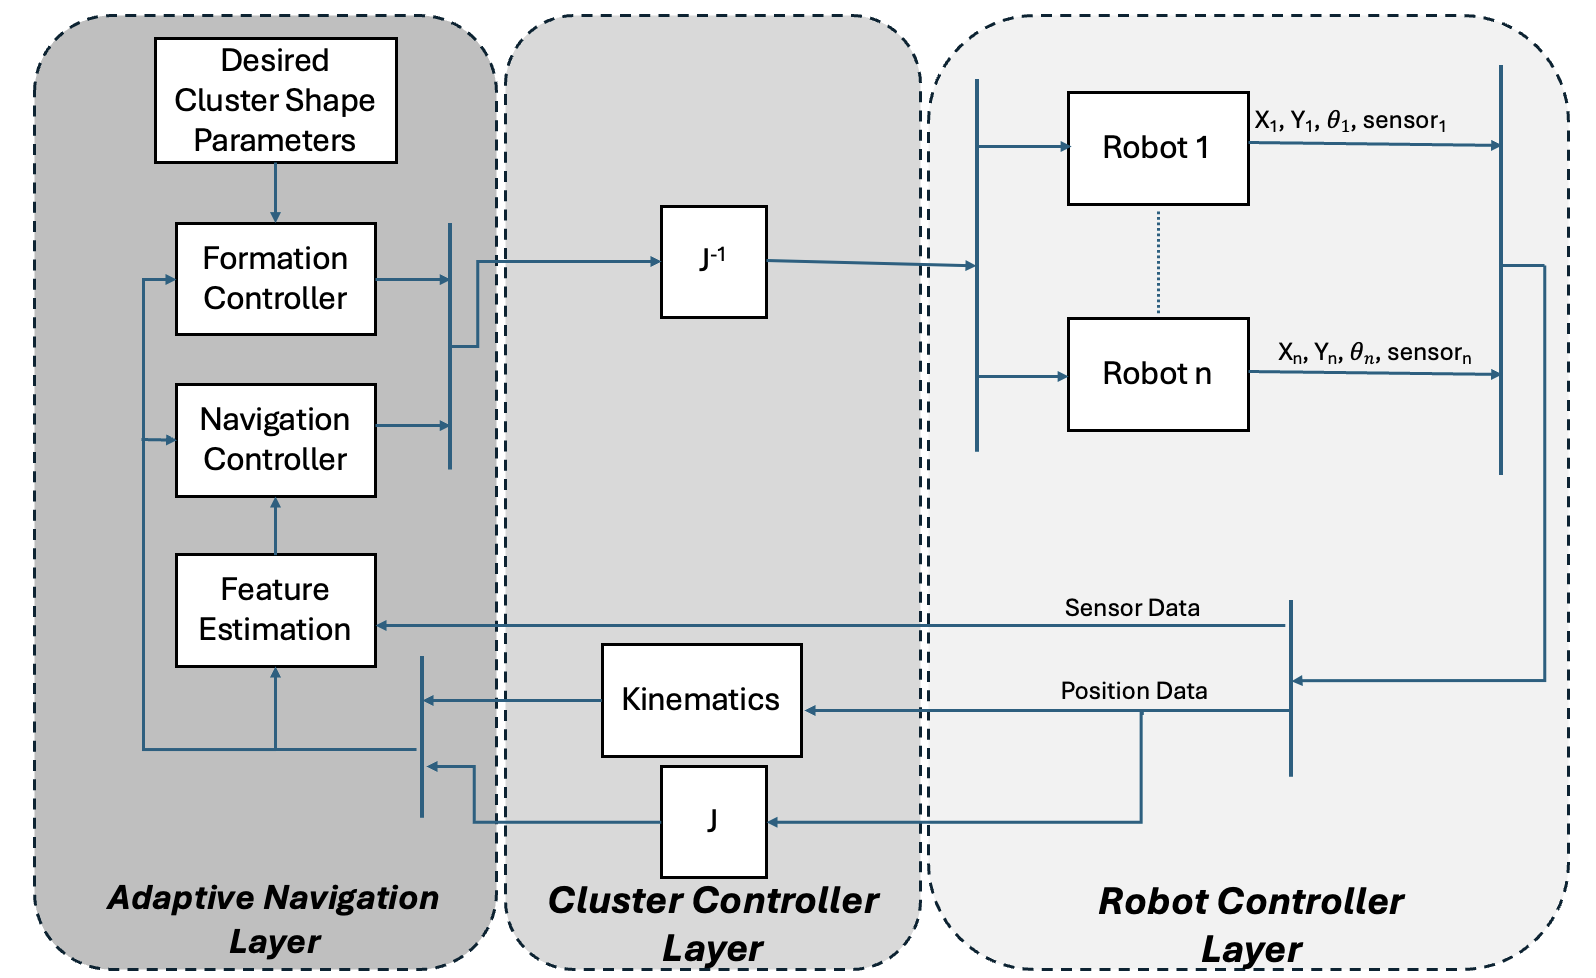
\includegraphics[width=0.32\textwidth]{figures/control_architecture.png}
    \caption{Three-layer control architecture. The adaptive navigation
    layer (left) estimates the field and generates the cluster command, the
    cluster controller layer (center) maps between cluster and robot space,
    and the robot controller layer (right) actuates each robot and reports
    its position and field sample.}
    \label{fig:control_architecture}
\end{figure}

\subsection{The $D$ Tracker}
\label{sec:sep_controller}

The $D$ tracker drives the centroid onto the trench of $D$ and then
along it, through the crest separating one saddle from the next.

A trench is taken here in the height-ridge sense. It is a curve on which the
gradient is orthogonal to a Hessian eigenvector whose eigenvalue is positive.
The surface is convex across the curve \cite{35}. The
derivation works in the eigenbasis of the estimated Hessian. Let
$\hat{\mathbf{H}}_{D,0}\mathbf{w}_k = \lambda_k \mathbf{w}_k$ with
$\|\mathbf{w}_k\| = 1$ and $\lambda_1 \leq \lambda_2$, taking
$\mathbf{w}_2$ across the trench and $\mathbf{w}_1$ along it, its sign
fixed by $\hat{\mathbf{v}}_0^\top \mathbf{w}_1 \geq 0$ to orient it
downstream. Identifying $\mathbf{w}_2$ with the trench normal is exact
on the benchmark, where $\mathbf{H}_D$ is diagonal
(Section~\ref{sec:dg_example}), and an
approximation in general.

The primitive below assumes a trench convex across and concave along,
$\lambda_1 < 0 < \lambda_2$. That is a property of the surface, not the
estimator, and it fails over the outer half of each separatrix segment
of the benchmark, where the true $\mathbf{H}_D$ is positive
definite (Section~\ref{sec:dg_example}).

$\hat{D}$ is an exact quadratic, so its Newton step
$-\hat{\mathbf{H}}_{D,0}^{-1}\hat{\mathbf{g}}_0$ reaches the fitted
stationary point in one move. The saturation of
Section~\ref{sec:arch} spreads that over several steps and bounds the
command as $\hat{\mathbf{H}}_{D,0}$ approaches singularity. The
stationary point is the crest, where the along-trench gradient vanishes,
so the Newton component is kept across the trench while the along-trench
direction comes from the ambient flow.

The along-trench command changes character where the trench levels off.
Away from a crest the along-trench gradient supplies a descent rate; at
one it vanishes, so the flow supplies the speed instead. That fallback is triggered inside a shallow-determinant band
$\mathcal{B}$, the set of points where
\begin{equation}
    |\hat{D}_0| < \varepsilon_{\mathrm{raw}}
    \quad\text{or}\quad
    \frac{|\hat{D}_0|}{\|\hat{\mathbf{H}}_{D,0}\|_F}
        < \varepsilon_{\dim},
    \label{eq:band}
\end{equation}
a raw threshold on absolute well depth, or a curvature-normalized one measuring depth against the local curvature. The latter carries units of length squared, so the band scales with the landscape rather than the absolute size of $D$. The band surrounds $\{D = 0\}$, not the separatrix, and that set also
contains the Okubo-Weiss boundary the cluster can cross during
acquisition. Triggering the condition there costs nothing, since the
along-trench speed passes to a flow that advects the cluster off-structure
while the transverse channel keeps acting. The
along-trench speed is
\begin{equation}
    v_\parallel =
    \begin{cases}
        \hat{\mathbf{v}}_0^\top \mathbf{w}_1,
            & \mathbf{p}_c \in \mathcal{B}, \\[6pt]
        \dfrac{|\mathbf{w}_1^\top \hat{\mathbf{g}}_0|}{|\lambda_1|},
            & \text{otherwise},
    \end{cases}
    \label{eq:vpar}
\end{equation}
and the velocity command is
\begin{equation}
    \dot{\mathbf{p}}_c =
    \underbrace{\mathrm{sat}(v_\parallel)\,\mathbf{w}_1}_{\text{along the trench}}
    + \underbrace{\mathrm{sat}\!\left(-\frac{\mathbf{w}_2^\top
      \hat{\mathbf{g}}_0}{\lambda_2}\right)\mathbf{w}_2}_{\text{across the trench}},
    \label{eq:d_law}
\end{equation}
scaled by the navigation gain $k$ of Section~\ref{sec:arch}.

This primitive decouples travel from trench holding through the eigenbasis.
The across-trench term is the Newton component of the fitted quadratic,
normalized by the transverse curvature $\lambda_2$. It is the same on and off
the band. The along-trench term takes its direction from $\mathbf{w}_1$, whose
arbitrary eigensolver sign is resolved against the measured flow to
point downstream. Since
$v_\parallel \geq 0$ in both branches, the
along-trench motion never opposes the ambient flow. At a crest the along-trench gradient vanishes while the separatrix
continues through, so the band test hands the speed to the flow.

When $\hat{\mathbf{H}}_{D,0}$ has eigenvalues of one sign the trench
frame is undefined, a case a general field will present and the primitive
must cover. Off the band it reverts to the signed Newton step
$\sum_k \mathrm{sat}(-\mathbf{w}_k^\top\hat{\mathbf{g}}_0/
\lambda_k)\mathbf{w}_k$, without a stability claim, and on the band to
the saturated flow alone. This fallback never fires on the benchmark,
for a reason specific to that field (Section~\ref{sec:disc_limits}), so
it is defined but untested.

That same sign test is the primitive's terminal condition. The cluster
holds when
\begin{equation}
    \lambda_1 \lambda_2 \geq 0,
    \label{eq:d_capture}
\end{equation}
when the fitted Hessian is no longer indefinite. Where two trench segments cross, at a flow saddle, the true $D$ has a local minimum and meets this test, the terminal analogue of the vanishing-gradient test the $s_1$ tracker uses.

Convergence follows from the trench geometry, for a cluster that realizes
$\dot{\mathbf{p}}_c$. Cluster space control tracks any commanded trajectory
with bounded error for unicycle robots \cite{37}, including those an
adaptive navigation layer generates \cite{2}, and the omnidirectional
robots here carry no nonholonomic constraint. The robot lag of
Section~\ref{sec:arch} is not modeled in what follows. In arclength coordinates $(\ell, n)$ along and across the trench, $D = h(\ell) + \tfrac{1}{2}\kappa_\perp n^2$ with $\kappa_\perp = 2\pi^6 A^2 > 0$ along a separatrix segment of the benchmark. The transverse channel of the $D$ tracker then reduces to $\dot{n} = -k\,\mathrm{sat}(a_\perp n)$, with $a_\perp = \kappa_\perp/\hat{\kappa}_\perp$ the ratio of true transverse curvature to fitted. Taking $V = \tfrac{1}{2}n^2$
gives $\dot{V} < 0$ for $n \neq 0$, so $|n|$ never grows. The cluster reaches the proportional region $|n| < c_{\max}/a_\perp$ in finite time and converges exponentially to the trench thereafter. Along the trench,
both branches of (\ref{eq:vpar}) keep $v_\parallel \geq 0$, so traversal
cannot reverse. Both branches also vanish at a stagnation point, where the flow and the
along-trench gradient go to zero together. The speed is therefore bounded
below only away from one. On a segment of length
$L_\Gamma$ excluding an $\varepsilon$ neighborhood of its endpoints the
realized speed satisfies $v_\parallel \geq m > 0$ and the segment is
crossed in time at most $L_\Gamma/(k\,m)$. The excluded neighborhood is
where the terminal test (\ref{eq:d_capture}) applies, and the transit
of it is bounded in the same way as the isotropic point of
Section~\ref{sec:s1_controller}. Bounded estimation error $\delta$ leaves the
trench practically stable at $\limsup |n| \approx \delta/(k\,a_\perp)$,
where the zero-mean part of the error spreads the tracking error and the
truncation bias displaces it instead.

\subsection{The $s_1$ Tracker}
\label{sec:s1_controller}

This primitive traverses the trench of $s_1$ using four quantities the
fit delivers, the eigenvalue $\hat{s}_1$, its gradient
$\nabla\hat{s}_1$, the strain eigenframe $(\mathbf{e}_1, \mathbf{e}_2)$,
and the deviatoric strain magnitude $r$, which measures how well resolved
that eigenframe is. No usable Hessian of $s_1$ exists
(Section~\ref{sec:surrogates}), so both channels are built from the
gradient.

The first step identifies the trench tangent. Naming an eigenvector
directly will not work, since $\mathbf{e}_1$ and $\mathbf{e}_2$ are
direction fields with no consistent sign, so the gradient is used. On
the trench the transverse derivative of $s_1$ vanishes by construction.
Away from a stationary point $\nabla\hat{s}_1$ points almost wholly along the trench. The tangent is whichever eigenvector the gradient is less orthogonal to.
\begin{equation}
    \mathbf{t}_{\mathrm{raw}} =
    \arg\max_{\mathbf{e} \in \{\mathbf{e}_1, \mathbf{e}_2\}}
    \bigl\lvert \nabla\hat{s}_1^\top \mathbf{e} \bigr\rvert,
    \qquad
    \mathbf{t} = \mathrm{sgn}\bigl(\mathbf{t}_{\mathrm{ref}}^\top
    \mathbf{t}_{\mathrm{raw}}\bigr)\,\mathbf{t}_{\mathrm{raw}},
    \label{eq:tangent_select}
\end{equation}
where $\mathbf{t}_{\mathrm{ref}}$ is the previous step's tangent once one
exists, or the measured flow $\hat{\mathbf{v}}_0$ on the
first tracking step. The rule selects $\mathbf{e}_2$ on the attracting
segment of the separatrix and $\mathbf{e}_1$ on the repelling segment, swapping
automatically through the origin (Fig.~\ref{fig:s1_channels}(a)).

The primitive alternates between traversing and settling, selected by a ride flag $\beta \in \{0,1\}$ that is one while traversing. The velocity command is
\begin{equation}
    \dot{\mathbf{p}}_c =
    \beta\,c_{\max}\tanh(1)\,\mathbf{t}
    - \mathrm{sat}\!\bigl(g_\perp\,\mathbf{P}\,\nabla\hat{s}_1\bigr),
    \qquad
    \mathbf{P} = \mathbf{I} - \beta\,\mathbf{t}\mathbf{t}^\top,
\end{equation}
where $\mathrm{sat}$ saturates a vector's magnitude and preserves its
direction, reducing to the scalar saturation on any multiple of a unit
vector.

\begin{figure}[!tb]
    \centering
    \includegraphics[width=0.48\textwidth]{figures/s1_channels.png}
    \caption{The two channels of the $s_1$ tracker, on the benchmark
    trench at $x = 0$. (a) Tangent selection,
    (\ref{eq:tangent_select}). At each sample the strain eigenframe is
    drawn, the selected eigenvector heavy and the rejected one light,
    with $\nabla\hat{s}_1$ in orange. The argmax takes
    $\mathbf{e}_2$ on the attracting segment and $\mathbf{e}_1$ on the
    repelling segment, swapping through the isotropic point at the origin.
    (b) The command. Travel along $\mathbf{t}$ is open loop at cruise
    speed, while $\mathbf{P}$ removes the along-trench component of the
    gradient so descent acts only across the trench. The along-trench
    slope of $s_1$ therefore does not drive the cluster toward a
    saddle.}
    \label{fig:s1_channels}
\end{figure}

This primitive decouples descent from travel through the projector
(Fig.~\ref{fig:s1_channels}(b)).
With $\beta = 1$, $\mathbf{P}$ removes the along-trench component of the
gradient, so the cluster descends only across the trench while riding
along it at cruise speed $c_{\max}\tanh(1)$. With $\beta = 0$ the
projector becomes the identity, the ride term drops out, and the same
expression is full gradient descent on $\hat{s}_1$, settling at a
local minimum. The gain $g_\perp$ is fixed and not
curvature-normalized, so the transverse channel contracts at gradient
rate.

The navigation controller moves $\beta$ through two transitions. It starts at zero and latches to one, beginning the ride, once $\hat{s}_1$ first falls below $-s_{\mathrm{trim}}$. That depth floor is a small fraction of the benchmark's well depth $-\pi^2 A \approx -0.987$ (Section~\ref{sec:dg_example}), so from most starting positions the latch sets at the first step, and the projected descent, not a separate homing phase, carries the cluster onto the trench. Terminal capture returns it to zero, holding the cluster at a two-dimensional
stationary point of $\hat{s}_1$ when
\begin{equation}
    r > r_{\mathrm{band}}, \qquad
    \lVert\nabla\hat{s}_1\rVert < g_{\mathrm{capture}}, \qquad
    \hat{s}_1 < -4 s_{\mathrm{trim}}.
    \label{eq:capture_test}
\end{equation}

A flow saddle is more than a crossing of two transverse trenches. It is
a true two-dimensional minimum of $s_1$, and on the benchmark this
is closed form, since (\ref{eq:s1_analytic_main}) gives
$s_1 \geq -\pi^2 A$ with equality exactly at integer $(x_f, y_f)$, a
strict nondegenerate minimum with curvature $\pi^4 A$ on both axes. The
full gradient therefore collapses there, while at an
ordinary trench point it remains large along the trench even
though it vanishes across it, so gradient magnitude alone distinguishes
the two. This matters because the ambient flow also stagnates at a
saddle, leaving any flow-based tangent rule without a direction exactly
where the ride needs one.
The three tests in (\ref{eq:capture_test}) reject, in order, the
isotropic point, an ordinary trench point, and a shallow flat spot away
from real structure. The $-4s_{\mathrm{trim}}$ depth
threshold is a hysteresis ratio, not a physical relation. The condition arms at four times the latch depth and releases when $\hat{s}_1$ rises back above $-s_{\mathrm{trim}}$. A noise-driven flicker of the gradient test does not send the cluster back through the tangent comparison at the well, while a real departure still does.

If the eigenframe is
degenerate, $r < r_{\mathrm{band}}$, and no previous tangent has been
established, then neither (\ref{eq:tangent_select}) nor continuity
supplies a direction. The command then rides the measured flow,
$\mathbf{t} = \hat{\mathbf{v}}_0/\|\hat{\mathbf{v}}_0\|$, with the
projector set to the identity. Only the first tracking step can reach
this case, and it is where the ambient flow enters the command.

The transverse argument is the same as for the $D$ tracker. The projector $\mathbf{P}$ at $\beta = 1$
removes the along-trench gradient, leaving the same transverse dynamics
$\dot{n} = -k\,\mathrm{sat}(a_\perp n)$, but with no curvature to
normalize by, the rate is set by the field, $a_\perp = g_\perp
\kappa_\perp(\ell)$, and $\kappa_\perp = \pi^4 A|\cos \pi y_f|$ vanishes
at the isotropic point at $y = 0$. The restoring force disappears there. So does the transverse gradient, so
nothing steers the cluster off the structure. The ride carries it across a ball of radius $\epsilon$ in time $2\epsilon/(k\,c_{\max}\tanh 1)$ while $|n|$ grows by at most $O(\epsilon)$, after which exponential convergence resumes. Traversal is immediate, since the tangential channel runs at constant speed with direction seeded once by the measured flow. That direction is guaranteed only under exact estimates.

\section{Simulation Program and Results}

\subsection{Simulation Setup}

A Python simulation of the architecture of Section~\ref{sec:arch} evaluates both primitives.
The double-gyre experiments use the steady field of
Section~\ref{sec:dg_example} ($A = 0.1$) on $[-1, 1] \times
[-0.5, 0.5]$. The integrator is explicit Euler with step $\Delta t = 0.1$ and robot dynamics follow the first-order model. The formation controller drives the nine shape terms to nominal proportionally (gain 1.0 on lengths, 0.1 on angles), and the cluster controller layer distributes the combined command through the analytic $12 \times 12$ inverse Jacobian. All trials use the nominal
formation with ring radius $\rho = 0.075$; a trial varies only the
formation's initial heading, drawn uniformly from $[0, 2\pi)$ in the
Monte Carlo sweeps and zero in the noise-free demonstration runs. The
cluster's angular velocity command is zero throughout, so
heading is held fixed at its draw, and ring-phase quantities are reported against it. Clean trials
run 400 to 600 steps and stop at domain exit or, for the $D$ tracker,
150 steps after first saddle contact. Noise-sweep trials run up to 500
steps and stop at task completion or domain exit. The
estimator-accuracy sweep holds the formation static and draws
independent noise per trial.

\subsection{Ocean HFR Setup}
\label{sec:ocean_sim}

The ocean experiment uses hourly surface-current frames for the Santa
Barbara Channel from the HFRNet U.S.~West~Coast Radial-to-Total Vector
product \cite{36}, on the $2$~km grid, which is public. The record is the one \cite{26} uses, the same network over the same 28-h window, 29 frames from May 16, 2012 08:00 GMT to May 17, 2012 12:00 GMT, so these results are interpretable against prior work on it. No controlled head-to-head was run, since initialization and advection differ.
Frames are interpolated linearly in time. World
coordinates on $[-0.65, 0.65]^2$ map affinely onto a region centered on
$(34.2^{\circ}\mathrm{N}, 120.4^{\circ}\mathrm{W})$.

Physical numbers follow from one unit block, length $L_w = 51.4$~km on
both axes and time $6000$~s, with a control period $\Delta t = 0.1$
time units, so one step advances the field by $600$~s and the
$168$-step trial covers the record. The commanded-speed cap
$\sqrt{2}\,k\,c_{\max}$ is then $0.87$~m/s, within reach of a small
autonomous surface vessel but above a buoyancy glider. The longitude
extent is
scaled by $\cos(34.2^{\circ})$, so both axes carry the same physical
scale and the map is a uniform dilation, so each zero set, trench, and
extremum of $D$ and of the strain eigenframe is the physical one. The
FTLE reference uses the same constants, so controller and evaluation
frames agree by construction. Those fields come from subwindows of this record at two
horizons. The 24-h field of Fig.~\ref{fig:ocean_ftle} integrates the
first 25 frames, and the four-anchor persistence check uses 12~h.

The pentagon is
enlarged to $\rho = 0.105$, $1.4\times$ the nominal radius and $5.4$~km
at this site, trading truncation bias for noise suppression so the
footprint spans about five cells of the $2$~km grid rather
than under four. At one control cycle per ten minutes any vessel time
constant is negligible, so $\alpha_{\text{mom}} = 0$, and the stiction
floor drops to $0.002$, having no vessel-scale analogue. No noise level is estimated for this field, since the exactly-determined six-robot fit leaves no residual to estimate $\sigma_{uv}$ from. Quantifying the uncertainty in ocean data is a harder problem, set aside here as in \cite{26}, so the noise model is validated on the double gyre only.

\subsection{Estimator Accuracy}
\label{sec:results_est}

\begin{figure}[!tb]
    \centering
    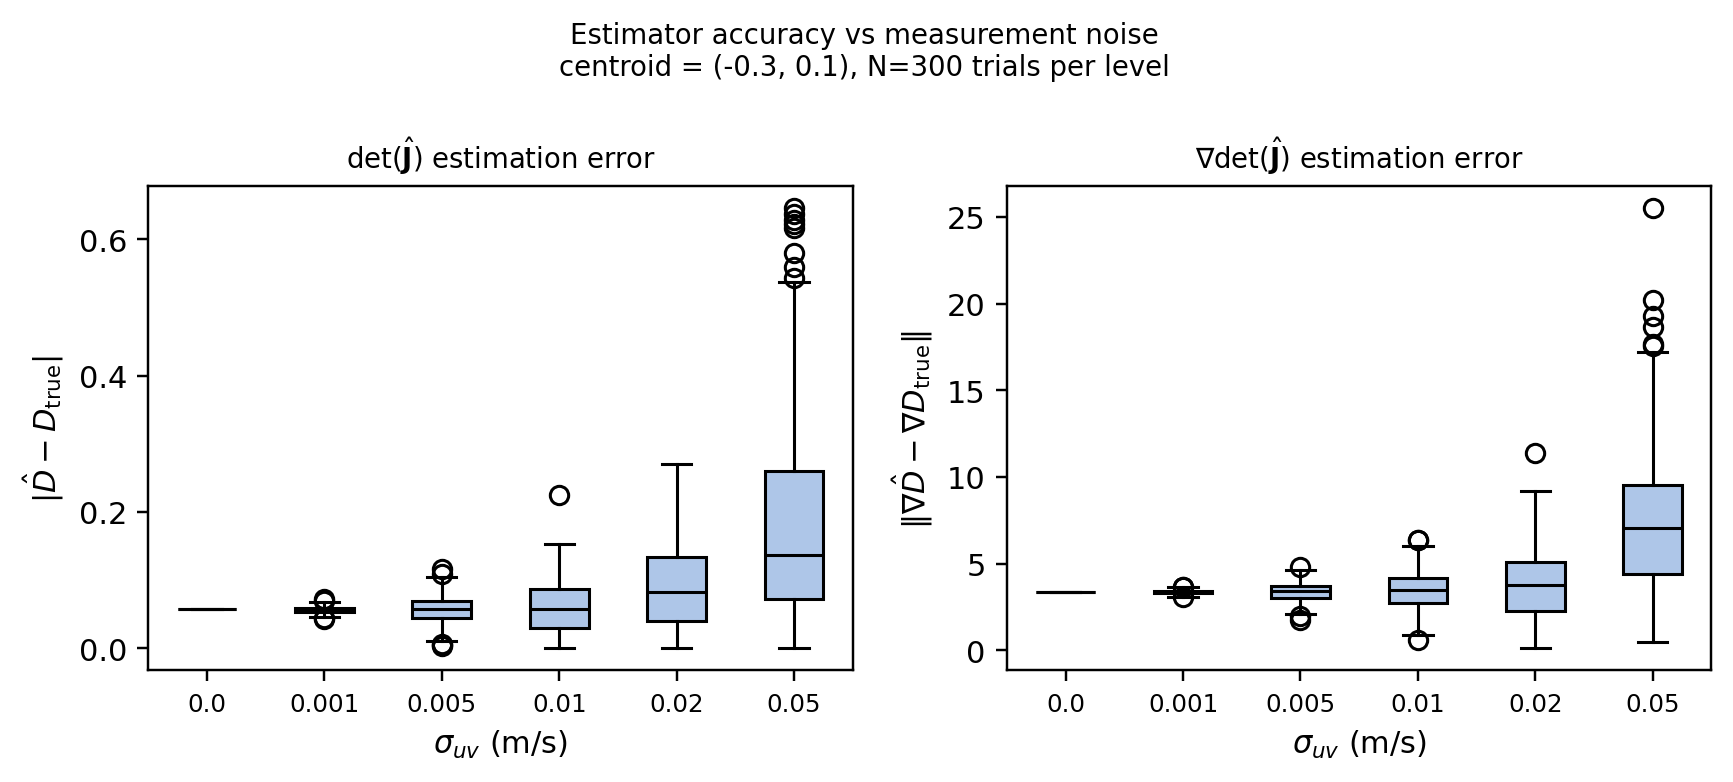
\includegraphics[width=0.68\columnwidth]{figures/estimator_accuracy_vs_noise.png}
    \caption{Estimator accuracy on the steady double gyre at the rotation-dominated
    point $(-0.3, 0.1)$, $10^4$ noise draws per point. (a) Median relative error
    of $\hat{D}$, $\nabla\hat{D}$, and $\hat{\mathbf{H}}_D$ against measurement
    noise at $\rho = 0.075$; the dashed line marks error equal to signal, the
    dash-dotted line the $D$ tracker's 50\% traverse-success level on the separatrix, for reference. (b) Mean
    angle between the fitted and true principal eigenvector of
    $\hat{\mathbf{H}}_D$, against the $45^\circ$ of a uniformly random axis.
    The star is truncation acting alone.}
    \label{fig:est_accuracy}
\end{figure}

The estimator was characterized on the steady double gyre before any
loop closed, over $10^4$ draws per condition at the rotation-dominated point
$(-0.3, 0.1)$, and the predictions of Section~\ref{sec:sensitivity}
held. The reading error induced
by position noise matched (\ref{eq:sigma_eff}) within 1.6\%. The downward bias of $\hat{s}_1$ matched (\ref{eq:s1_bias}) within 5\% in eighteen of twenty-four conditions, and within one standard error in all twenty-four. The six wider cases sit at $r/\sigma_r \geq 3$, where the predicted bias falls below the resolution of $10^4$ draws. The
signed mean error of $\hat{D}$, $\nabla\hat{D}$, and
$\hat{\mathbf{H}}_D$ was zero to within 2.7\% of one standard deviation
across forty-eight conditions, as measurement-noise unbiasedness
requires. The correlation between the two component errors at one robot
was $0.41$ under position noise against $0.44$ predicted, and zero
under measurement noise, the mechanism separating the
channels.

In Fig.~\ref{fig:est_accuracy}(a), $\hat{D}$ stays informative to
$\sigma_{uv} \approx 0.07$ and $\nabla\hat{D}$ to $\approx 0.0075$, while
$\hat{\mathbf{H}}_D$ never clears the error-equals-signal line at any
noise level, bottoming at $0.94$. In Fig.~\ref{fig:est_accuracy}(b),
truncation acting alone costs the $\hat{\mathbf{H}}_D$ eigendirections
$2.2^\circ$, while noise costs them $24^\circ$ by $\sigma_{uv} = 0.003$ and
$39^\circ$ at the closed-loop failure cliff, against $45^\circ$ for a
uniformly random axis.

The $s_1$ channel was checked at the nominal radius against its analytic
values. The fitted shear strain is at the $10^{-4}$ level against an
analytic zero, and the fitted $\hat{\mathbf{H}}_{s_1}$ eigenvalues are
negative semidefinite as Section~\ref{sec:surrogates} requires. The
transverse component of the fitted gradient at $(0.03, 0.25)$, averaged
over ring phase, recovers a restoring slope of $6.83$ against the
analytic $6.888$, a $0.9$\% truncation deficit. Rotating the ring
through its $72^\circ$ period moves that slope between $4.0$ and $9.7$,
and halving $\rho$ halves the spread, confirming the linear-in-radius
scaling. The mean tracks the analytic value, so averaged over heading the estimator is not
biased in the transverse channel, though at any single heading it is. At $\sigma_{uv} = 0.01$ the median direction error of
$\mathbf{e}_2$ is $4.5^\circ$, against $44^\circ$ for $\nabla\hat{s}_1$
and $41^\circ$ for the $\hat{\mathbf{H}}_D$ eigenvector.

\subsection{Clean Runs}
\label{sec:disc_clean}

\begin{figure*}[!tb]
    \centering
    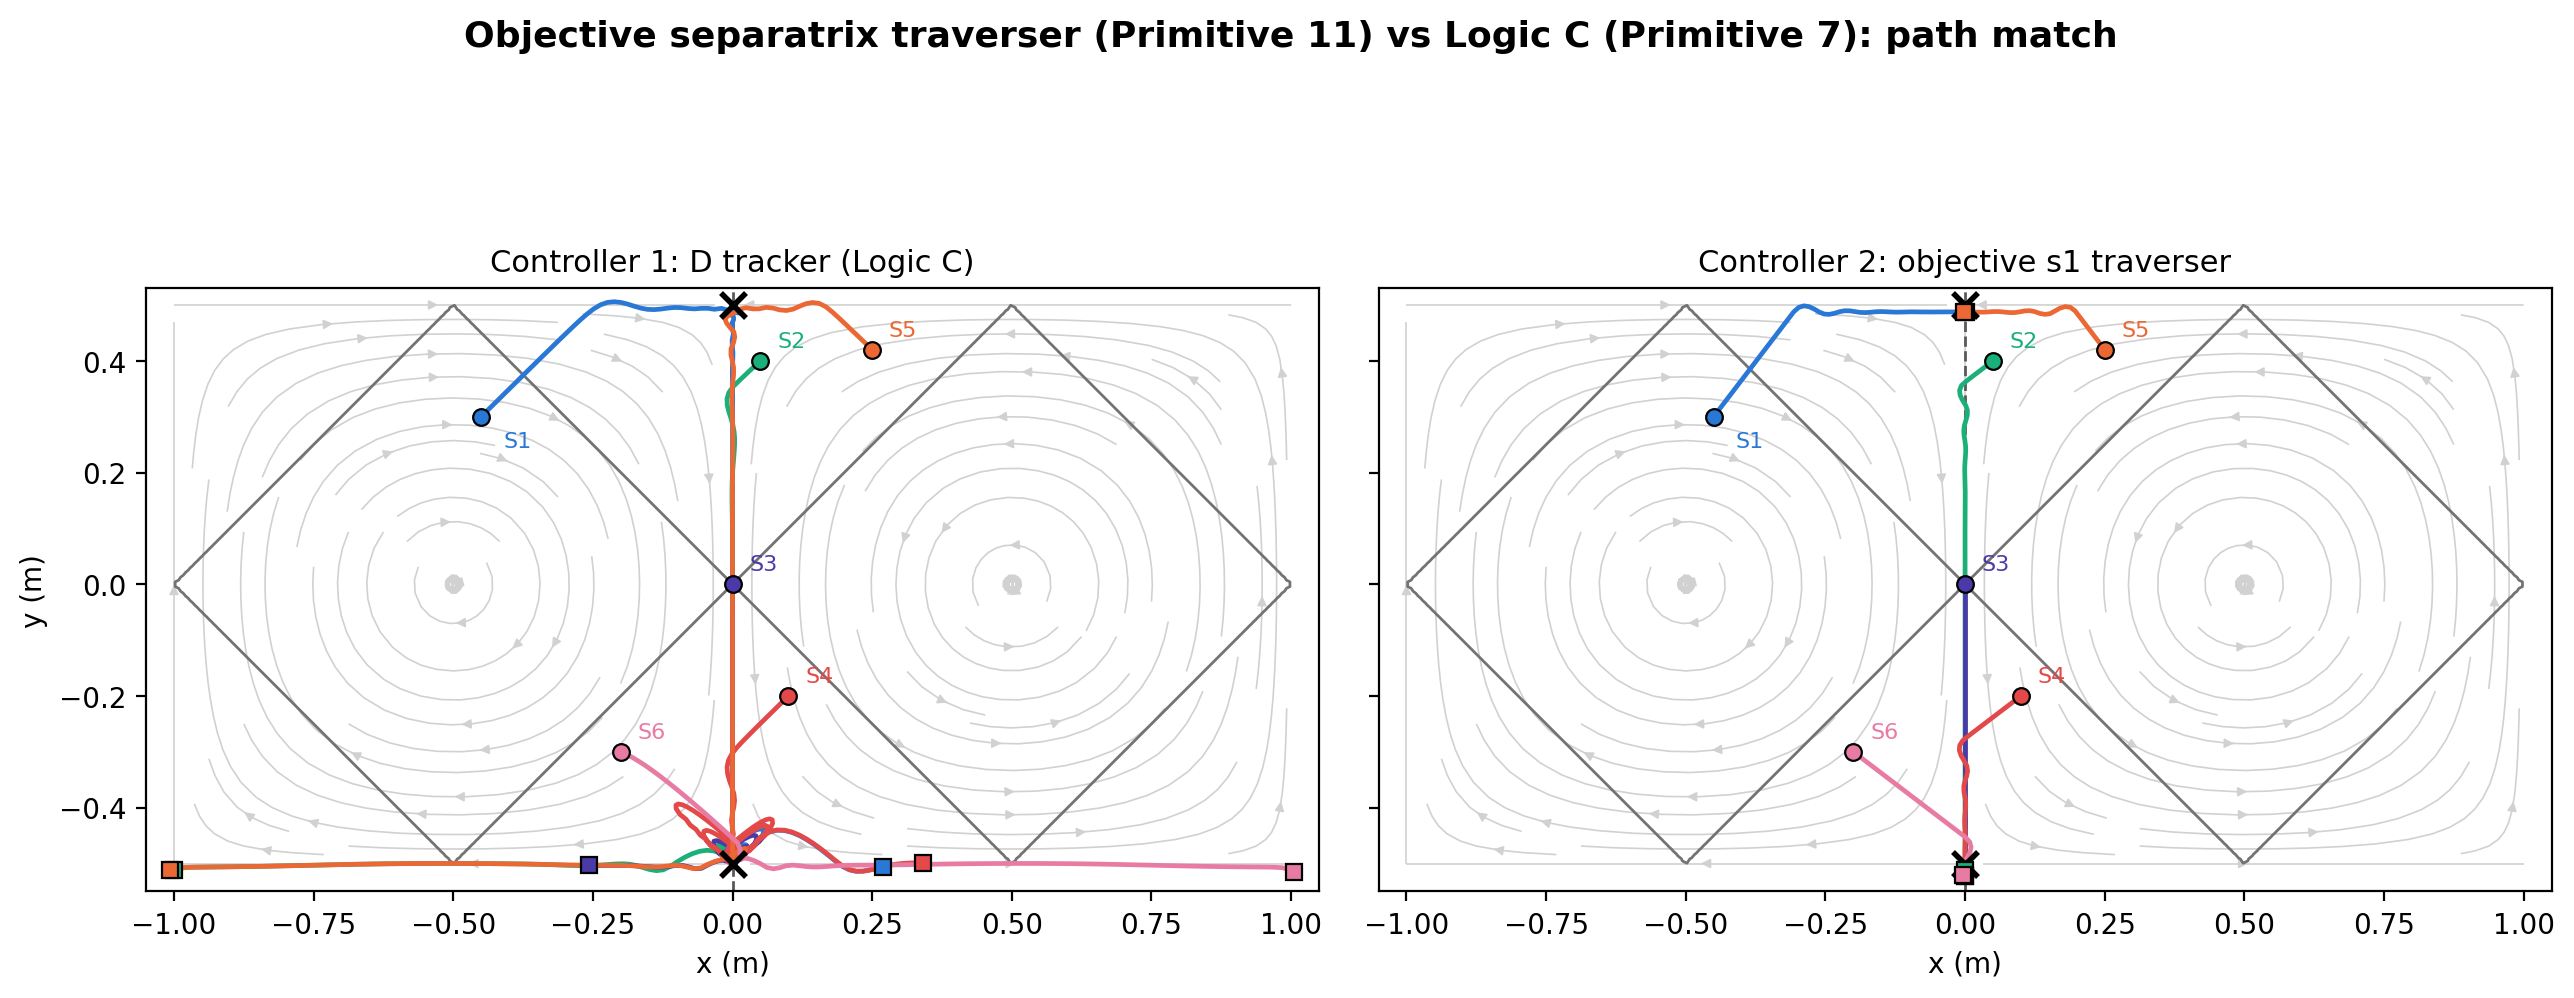
\includegraphics[width=0.92\textwidth]{figures/traverse_vs_logic_c.png}
    \caption{$s_1$ tracker versus $D$ tracker from six matched starts
    ($\bullet$), noise-free, overlaid on the double-gyre streamlines and
    Okubo-Weiss diamonds. Both traverse the same network through the
    isotropic point at the origin. The $s_1$ tracker captures at the
    saddle ($\times$) its tangent orientation resolves toward, while the
    $D$ tracker continues onto the crossing wall trench past each saddle
    it reaches, ending at the square markers.}
    \label{fig:traverse_vs_logic_c}
\end{figure*}

These runs test acquisition, traversal, and the terminal step for both primitives. On the double gyre the two fields share every trench (Section~\ref{sec:dg_example}).

Both ran noise-free from six matched starts
(Fig.~\ref{fig:traverse_vs_logic_c}), spanning both gyre halves, the origin, and points up to $2.7\rho$ off the structure, acquiring the network from all six in 0 to 35 steps for the $D$ tracker and 0 to 46 for the $s_1$ tracker. They then ride the same segments in the same direction and cross the isotropic point at the origin. A run
acquiring above the origin therefore rides an attracting OECS to that
point and continues onto a repelling one, on the same primitive and the
same scalar trench throughout. Neither needs a dedicated rule at the
crossing. The $s_1$ tracker rides through the origin on ordinary tangent
selection, and over a sweep of $r_{\text{band}}$ from 0.05 to 0 the
degenerate-frame fallback never fires once.

The primitives part only at the terminal step, and the split follows
from what each surrogate has at a saddle. The $s_1$ tracker
settles within 0.011 to 0.022 of a saddle in all six runs, at whichever
its initial tangent resolves toward, four at
$\mathbf{p}^*_1 = (0, -0.5)$ and two at $\mathbf{p}^*_2 = (0, 0.5)$. The
$D$ tracker passes within 0.02 of $\mathbf{p}^*_1$, then rides onto the
crossing wall trench and continues, because the capture test
$\lambda_1\lambda_2 \geq 0$ cannot fire. The field has
$u_{xx} = u_{yy}$ and $v_{xx} = v_{yy}$, so the fitted
$\hat{\mathbf{H}}_D$ is traceless here up to truncation error, and its
eigenvalues approximate $\pm|\hat{H}_{xx}|$. At the cluster's $0.05$
offset from the well the estimated pair is $[-0.51, 0.45]$ against a
true $[18.3, 19.2]$. The second derivatives of the field vanish at the
saddle, so the true pair comes mostly from products of the Jacobian with
third derivatives, which a quadratic fit omits, and the induced trace is
a finite-radius truncation artifact. The same underestimate also
carries the cluster through, since the off-band along-trench speed
(\ref{eq:vpar}) divides by $|\lambda_1|$ and a fitted $0.51$ against a
true $18.3$ inflates it by a factor of order thirty.

This limit applies to both surrogates. $\hat{\mathbf{H}}_{s_1}$ is negative
semidefinite for every field and formation (Section~\ref{sec:surrogates}), so
neither surrogate admits a definiteness certificate. The one terminal test a quadratic fit supports is a vanishing gradient. The fitted \emph{gradient} tracks the true gradient even where the fitted \emph{curvature} carries the wrong sign, and a flow saddle is a true two-dimensional minimum of $s_1$. The test is
therefore sufficient where the $s_1$ tracker needs one. However, it is
unavailable where the $D$ tracker would need one.

Acquisition does not depend on the start. Over a 20\,000-cell
start-position grid no run settles at a gyre center, since descent of
$\hat{D}$ leaves the rotation-dominated interiors instead of stalling in
them.


\subsection{Behavior Under Noise}
\label{sec:disc_noise}

\begin{figure}[!tb]
    \centering
    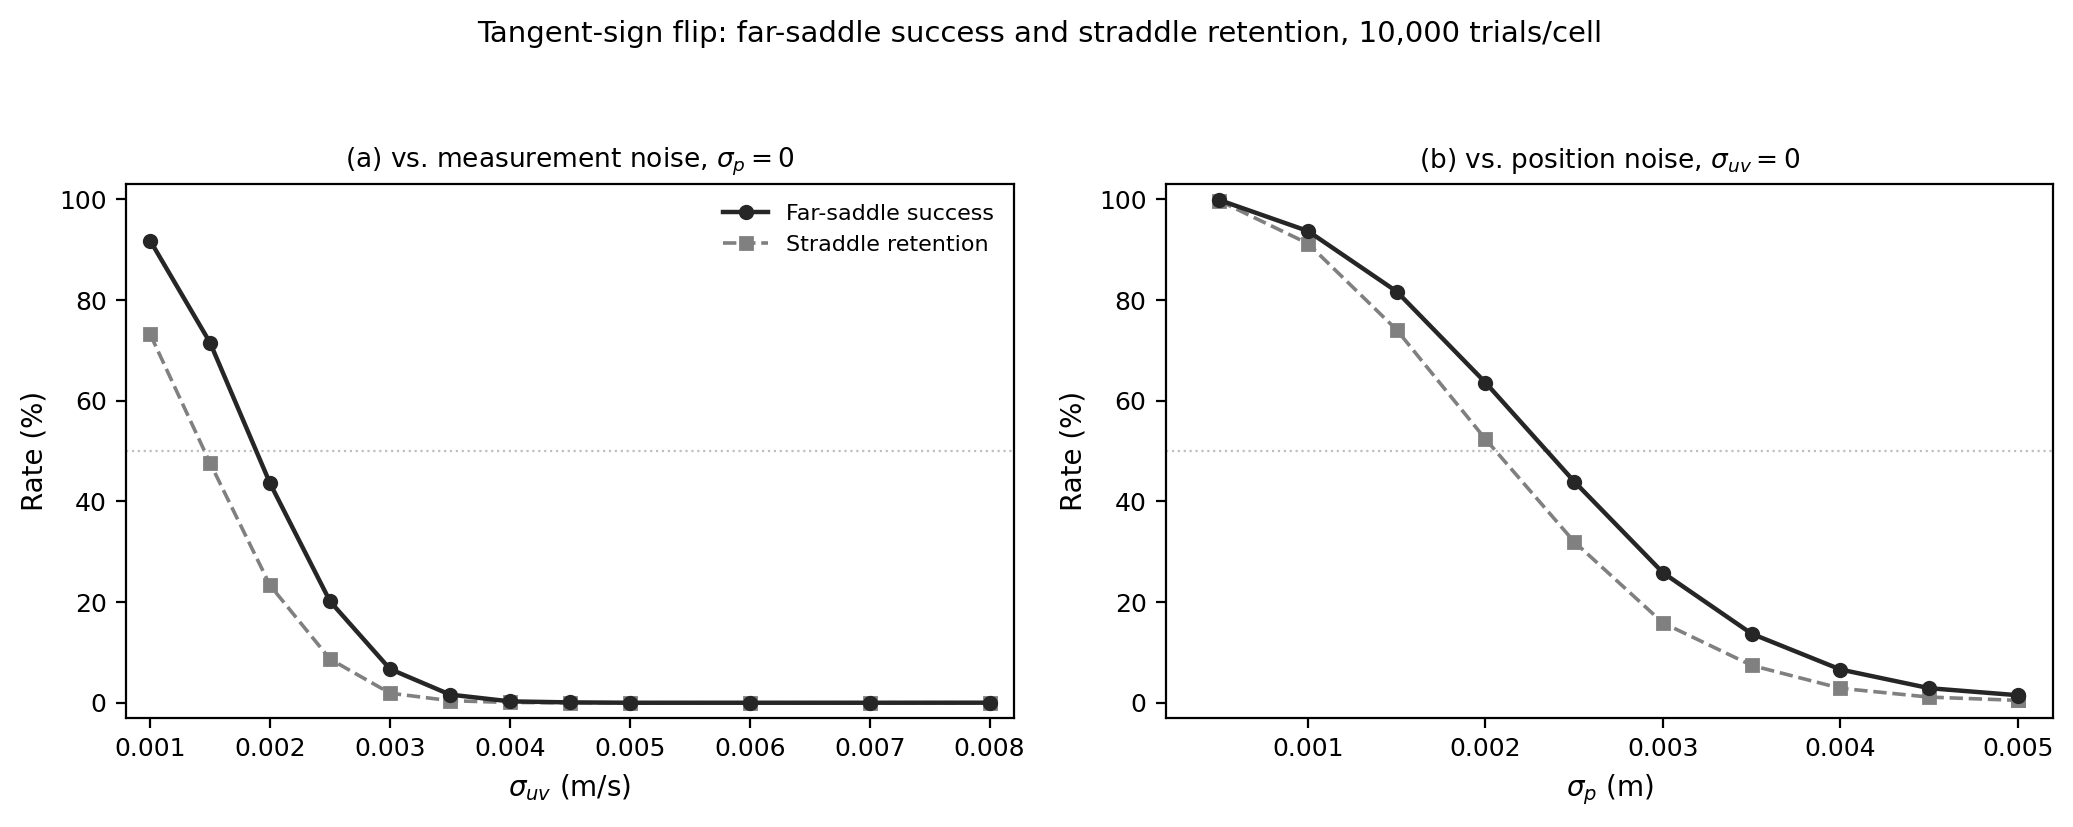
\includegraphics[width=0.68\columnwidth]{figures/flip_resolution.png}
    \caption{Resolving the $s_1$ tracker's tangent-sign flip. Far-saddle success and
    straddle retention (both conditioned on reaching $\mathbf{p}^*_1$),
    10\,000 trials/cell, at 0.0005 spacing on each axis. (a) Against
    $\sigma_{uv}$, $\sigma_p = 0$. (b) Against $\sigma_p$,
    $\sigma_{uv} = 0$.}
    \label{fig:flip_resolution}
\end{figure}

Both primitives sweep the same two-dimensional noise grid from one
straddling start, $(0, 0.35)$, at 10\,000 trials per cell from
independent headings. Success is contact within 0.06 of the far saddle $\mathbf{p}^*_1 = (0, -0.5)$, which a noise-free run from this
start reaches under either primitive, without formation collapse; each trial
also records straddle retention and tracking error. A trial straddles when the robots fall on both sides of the separatrix,
and retention requires it never stop once started, the failure
\cite{26} reports. Holding one target fixed makes a settle at the near saddle a
directional failure rather than a loss of the structure. Both succeed in every noise-free trial. Noise separates them in favor
of the $D$ tracker, whose 50\% crossing sits at
four to five times the $s_1$ tracker's, and the two fail differently.

For the $D$ tracker the cliff sits where the estimator runs out. Success crosses 50\% at $\sigma_{uv} \approx 0.0079$. Along the separatrix between $y = \pm 0.35$, $\nabla\hat{D}$ stops being informative between $\sigma_{uv} \approx 0.0047$ and $0.0085$, a range that brackets the cliff, and at the cliff the curvature eigenframe is $32^\circ$ to $40^\circ$ from truth against $45^\circ$ for a random axis. Both terms of the $D$ tracker are built on that frame.

The $s_1$ tracker crosses 50\% between $\sigma_{uv} = 0.0015$ and 0.002
(Fig.~\ref{fig:flip_resolution}). These cliffs are 2.5\% and 0.5 to 0.6\% of the peak speed $\pi A$, below what trackers steering on raw velocities tolerate \cite{26,30}, since this estimator differentiates the field twice. On the separatrix $s_s \equiv 0$ and $\mu \equiv 0$, so the gradient collapses to $\nabla\hat{s}_1 = \pm(\hat{a}_5, \hat{a}_4)$ and tangent selection reduces to the comparison $|\hat{a}_5| > |\hat{a}_4|$. The true $a_5 = u_{xx}$ is identically zero there and $a_4$ collapses at both saddles, so the comparison decides at a signal-to-noise ratio of $1.4$ at $\sigma_{uv} = 0.002$, against the seed's $71$. Supplying one channel at a time confirms it. A clean flow to the seed
moves the correct-saddle rate at $\sigma_{uv} = 0.002$ from 44.6\% to
45.8\%, and a clean gradient and eigenframe to the argmax moves it to 100\%. The cluster settles in the wrong direction, a sign inversion.

Formation radius trades robustness against accuracy. A sweep over
$\rho \in \{0.0375, 0.075, 0.105, 0.15\}$ at 400 trials per cell found
far-saddle success rising with $\rho$ for both trackers at every noise
level, while the zero-noise tracking error roughly doubled between
$\rho = 0.075$ and $0.15$, from 0.0016 to 0.0031 for the $D$ tracker and
from 0.0075 to 0.0145 for the $s_1$ tracker.

The zero-noise tracking errors, 0.0075 for the $s_1$ tracker against 0.0016 for the $D$ tracker, do not come from noise. Both primitives park where their own transverse command vanishes, on the \emph{fitted} trench rather than the field's, and the offset between the two is the orientation-dependent truncation bias. Noise robustness depends less on per-cycle estimation accuracy than on how long a sign decision persists before a new measurement checks it. The $D$ tracker re-signs $\mathbf{w}_1$ against $\hat{\mathbf{v}}_0$ every cycle; the $s_1$ tracker carries the sign in state through $\mathbf{t}_{\text{ref}}$. That reliance follows from objectivity and traversal together. Objectivity rules out the fitted curvature (Section~\ref{sec:surrogates}), the measured flow (Appendix~\ref{app:equivariance}), and a world axis as sign references, and traversal rules out the along-trench component of $\nabla\hat{s}_1$, which reverses at the along-trench maximum the ride must cross, leaving the
primitive's own prior output.

\subsection{Behavior Under a Rotating Observer}

\begin{figure}[!tb]
    \centering
    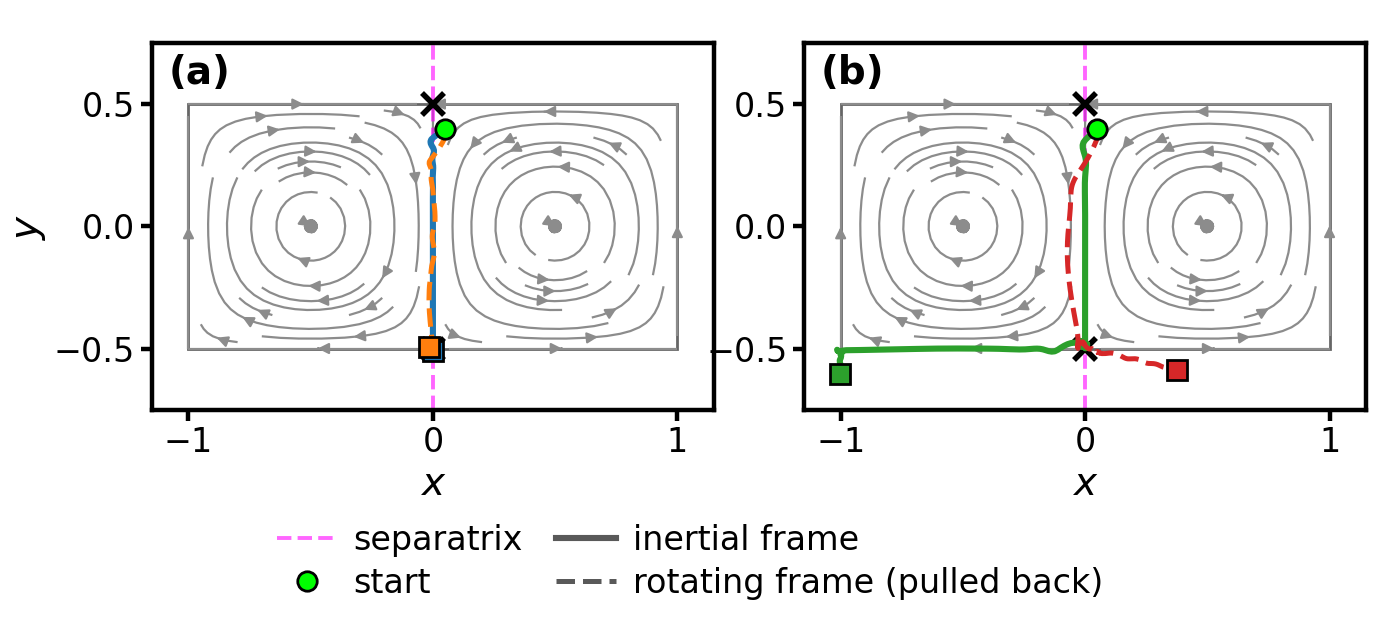
\includegraphics[width=0.95\columnwidth]{figures/objectivity_traverser.png}
    \caption{Objectivity trial, both primitives started from
    $(0.05, 0.40)$ and run in the inertial frame (solid) and in a
    frame rotating at $\Omega = 0.2$ (dashed, pulled back to
    inertial coordinates). (a) the $s_1$ tracker's two runs coincide
    and capture at the same saddle (final gap
    0.025). (b) the $D$ tracker's rotating-frame run leaves the
    separatrix (final gap 1.219), the artifact predicted by
    (\ref{eq:D_not_objective}).}
    \label{fig:oecs_objectivity}
\end{figure}

Both primitives were run from $(0.05, 0.40)$, just inside the upper
saddle, on the same physical double gyre in two observer
frames, the inertial one and a frame rotating at $\Omega = 0.2$, where the field is $\mathbf{v}'(\mathbf{p}', t) =
\mathbf{Q}\mathbf{v}(\mathbf{Q}^\top \mathbf{p}') + \Omega\,(-y',
x')^\top$. At a Rossby number $\mathrm{Ro} =
\lvert\omega\rvert_{\max}/2\Omega \approx 4.9$ the frame perturbs the
vorticity scale. The rate keeps the structure's apparent speed
at the tracked radius, $\Omega r \leq 0.10$, inside the command
authority $k\,c_{\max} = 0.12$, the condition the appendix requires.
Rotating-frame trajectories are pulled back to inertial coordinates and
compared with the inertial run of the same primitive.

The $s_1$ tracker's two runs (Fig.~\ref{fig:oecs_objectivity}) are the same material path, final gap 0.025 and mean gap 0.014, both capturing
at the same bottom saddle. The $D$ tracker's rotating-frame run leaves the structure, reaching a mean trench-network
distance ten times its inertial value of 0.005 and a final gap of 1.219
from the inertial run. Trench-network
distance is the run-averaged distance from the centroid to the nearest
line of the benchmark's trench grid, $x \in \{-1, 0, 1\}$ and
$y = \pm 0.5$.

The added solid-body vorticity moves the whole $D'$ landscape, and the same rotation adds a transport term to the measured flow, which signs $\mathbf{w}_1$ every cycle and sets the on-band speed. Both terms of the $D$ tracker are steered by a frame artifact rather than by the field. The artifact is in the surrogate, and against $D$
itself it is unbounded at the crest the primitive must cross. The $s_1$ tracker is covered instead by
Appendix~\ref{app:equivariance}, which exempts one instant and
holds only up to the frame-transport term that the 0.025 gap measures.

\subsection{Behavior on a Measured Field}
\label{sec:disc_ocean}

\begin{figure}[!tb]
    \centering
    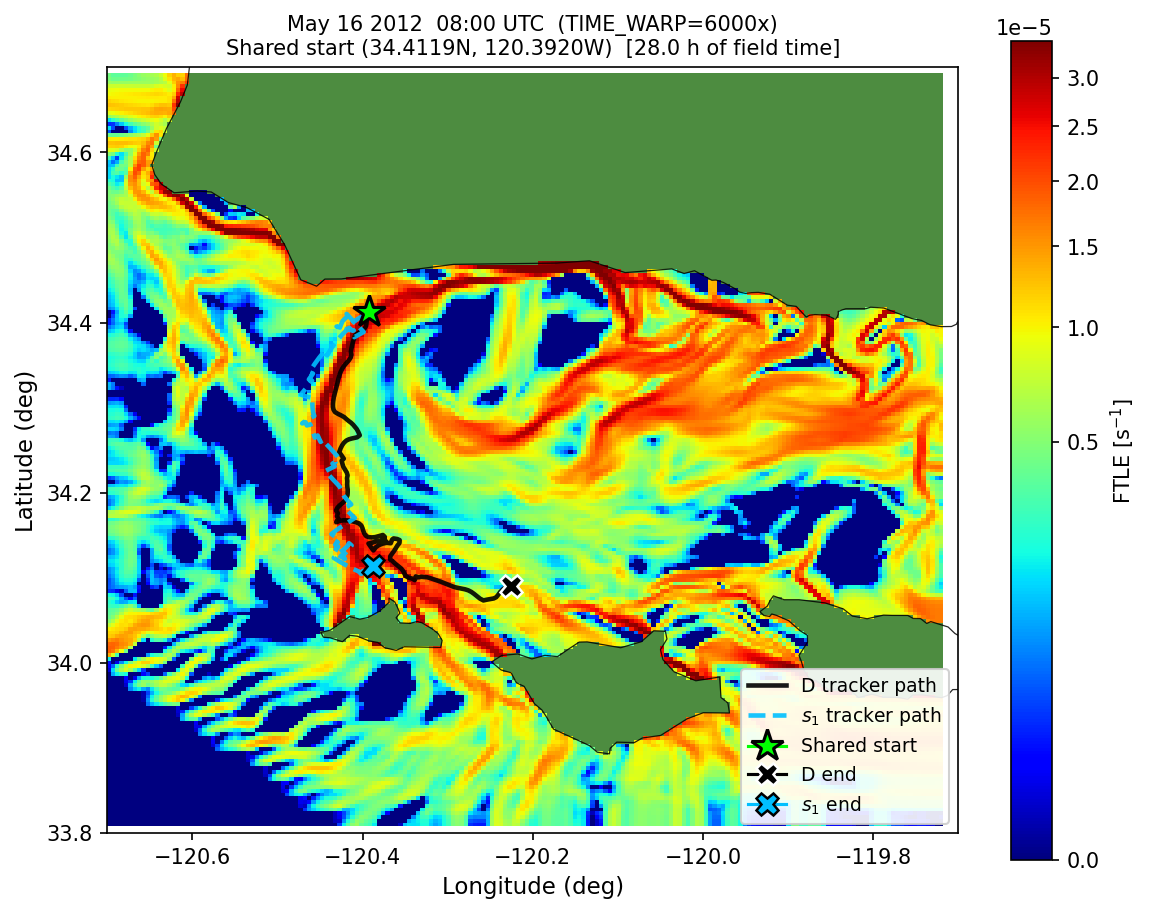
\includegraphics[width=0.30\textwidth]{figures/ocean_ftle_trajectory_overlay_2km.png}
    \caption{28-h $D$ and $s_1$ tracker paths, from a single shared
    start, over the 24-h forward FTLE field computed offline from the
    same 2~km data and anchored at the record start. Both follow the
    dominant ridge from the channel entrance to the bifurcation and
    separate only near landfall.}
    \label{fig:ocean_ftle}
\end{figure}

A measured field has no reason to carry a vorticity-free trench
network, so nothing forces the two surrogates
onto a common curve. It also carries nonzero horizontal divergence, so $s_1 + s_2 = 2\mu$ no
longer vanishes. That departure, $2|\mu|/r$, normalizes the divergence against the deviatoric strain. It has median $0.8$--$1.1$ and 90th percentile $3.0$--$5.9$ along the two
primitives' paths. The $s_2 = -s_1$ substitution is therefore not tightly
bounded here, and the $D = -s_1^2$ reading of their agreement is
qualified accordingly.
Both were run unmodified from a shared start north of the channel
entrance, $(34.41^{\circ}\mathrm{N}, 120.39^{\circ}\mathrm{W})$, at
the operating point of Table~\ref{tab:params}. The $s_1$ tracker's depth condition latched at the first step and stayed
latched for the entire 168-step run. The record therefore reports the ride,
not gradient descent on an unlatched field. Both spend the record near the edge
of their command authority, the $D$ tracker reaching the $0.87$~m/s cap
exactly against a $0.71$~m/s mean, and the formation stays far from the
conic degeneracy throughout, at its nominal $\kappa(\boldsymbol{\Phi}) = 8.26$. Over the 28~h trial both descend through the channel entrance and track the same ridge through the bifurcation, separating only at the end, where the $D$ tracker makes landfall on the middle island.
Because the field is time-varying, the navigation gain sets how fast
the cluster arrives at the bifurcation and so which branch of the
evolving ridge it meets, the branch $k = 1.8$ selects.

Fig.~\ref{fig:ocean_ftle} places both trials against the 24-h forward-time
FTLE field, computed offline in the style of
\cite{15}. Both follow the dominant ridge from the channel entrance to the
bifurcation closely. Mean distance from the tracked path to the nearest 95th-percentile ridge point
is 1.8~km for the $D$ tracker and 2.4~km for the $s_1$ tracker. The grid is
2~km and the formation radius 5.4~km. That ridge was available to neither. Forward FTLE recomputed at four anchor times confirms that the dominant ridge
persists while the finer structure downstream evolves. The $D$ tracker's branch
outcome agrees across 84 of 100 jittered starts.

The double gyre is a
special case with a vorticity-free trench network
(Section~\ref{sec:surrogates}), and this is a finding
on one record rather than a guarantee that carries to arbitrary flows. The record is also time-varying,
each primitive seeing only instantaneous samples at its own position,
with no analytic guarantee.

The ocean field's degeneracies are isolated and its eddy centers move between frames. The trial
therefore exercises tangent selection where neither the eigenframe nor the
trench network is axis-aligned, which the double gyre cannot do. It offers no
two-dimensional minimum of $s_1$ within reach of the ride, so the
capture test, which is always armed, never engages and the same
unmodified primitive behaves as a traverser.

\subsection{Limitations}
\label{sec:disc_limits}

Cluster space control is centralized, requires global state, becomes intractable
for suitably large clusters, and is impractical without reliable
high-bandwidth communication among the robots \cite{31}. The claims here
are for small clusters in a limited workspace with ample bandwidth, the
regime the six-robot estimator occupies. Computation is not a constraint
here, at one $6 \times 6$ solve per cycle against a $600$~s ocean step.

Two limitations sit in the estimator and its band logic. The fit is
ill-conditioned whenever the six sampling points drift toward a common
conic, and no field tested here drives the formation toward one, so the
estimator is untested in the regime its own conditioning limit
describes; the mitigation, monitoring $\kappa(\boldsymbol{\Phi})$ with a
shape-maintenance term, is not implemented. The band test carries no
hysteresis, so noise can chatter the $D$ tracker across its boundary,
which costs speed alone, since both branches share the same transverse
dynamics.

The $s_1$ tracker has two weaknesses where $\mathbf{S}$ approaches isotropy. The first is the $1/r$ term of (\ref{eq:s1_bias}). Tangent selection is the
defense once the ride is underway, and the residual risk of a wrong
branch at a crossing under heavy noise is damped but not excluded by the
capture test latch. The second is the eigenvector comparison, which remedies aimed at the seed do not reach (Section~\ref{sec:disc_noise}).

The $D$ tracker's traversal past a saddle is untested off the benchmark,
and on it runs outside the premise of
Section~\ref{sec:sep_controller}. Where the true $\mathbf{H}_D$ is
positive definite the degenerate-frame fallback should fire and does
not, because $u_{xx} = u_{yy}$ and $v_{xx} = v_{yy}$ on this field
leave (\ref{eq:hess_det}) traceless up to truncation error, too small to
separate the eigenvalue signs.

No controlled head-to-head against the straddle family \cite{26,27,28} or the onboard-FTLE strategy of \cite{30} was run. Running those methods from an off-structure start is outside their stated problems, and their robots are advected while this paper's are not, so one simulator cannot host both.
All results are simulated, and the ocean run samples the gridded product without added noise. The no-advection premise is exact for the
planned Decabot follow-on, where the field is encoded and read rather
than physically experienced \cite{34}, but on the ocean field it is an
extrapolation, untested against real advection.

\section{Conclusion}

This paper has shown that a second-order fit of the local flow, from six
robots sampling at once, is enough to acquire and ride the instantaneous
coherent structures of a planar flow. The fit gives the velocity gradient
as a field over the formation, and the two adaptive navigation primitives
built on it use only synchronous local velocity measurements, with no
map, no forecast, and no assumption about the structure's identity. Both
present the same interface to the cluster controller layer.

The experiments give an operational selection rule. With a noisy sensor
the $D$ tracker withstands four to five times the noise the $s_1$ tracker does. Under a rotating observer the
ranking reverses. The $D$ tracker leaves the structure, final
gap 1.219, while the $s_1$ tracker returns the same material curve in
both frames, final gap 0.025. On Santa Barbara Channel currents both followed the same transport corridor
for 28 hours, at mean distances of 1.8 and 2.4~km from an FTLE ridge neither could see. A cluster that can certify its orientation should carry the $D$ tracker,
which tolerates a noisier sensor. One that cannot should carry the $s_1$ tracker, which is objective.

Ongoing and future work targets a) extending the stability results to
time-varying fields; b) online formation reshaping, to protect the
conditioning of $\boldsymbol{\Phi}$ and average out the truncation
bias; c) a cubic fit from ten robots off any common cubic curve, which
recovers the third derivatives on which the true $\mathbf{H}_D$ and the
transverse curvature of an $s_1$ trench depend; and d) verifying both
primitives on the Decabot testbed and then with surface vessels.

\appendices

\section{Frame Equivariance of the $s_1$ Tracker}
\label{app:equivariance}

Let an observer rotate as $\mathbf{p}_Q = \mathbf{Q}(t)\mathbf{p}$. The
strain tensor co-rotates and $s_1$ and $r$ stay invariant
(Section~\ref{sec:surrogates}), while the eigenframe and $\nabla s_1$
turn with the frame. Both tests the $s_1$ tracker performs, tangent
selection and the capture test, are scalar inequalities in those
invariants, so each returns the same verdict in every frame and the
command is equivariant, $\boldsymbol{\delta}_Q = \mathbf{Q}\boldsymbol{\delta}$.

Equivariant commands do not by themselves give equivariant paths. A
rotating observer integrates $\dot{\mathbf{p}}_Q = k\boldsymbol{\delta}_Q$,
while the transported inertial path picks up the frame's transport
velocity, so the two separate at rate $\Omega\lVert\mathbf{p}_Q\rVert$.
That difference enters the transverse channel as a bounded disturbance,
so provided the frame turns slower than the cluster can correct,
$\Omega\lVert\mathbf{p}_Q\rVert < k\,c_{\max}$, the residue does not
accumulate and the tracker follows the same structure in every frame.

One step is exempt. The tangent is seeded once, when the ride begins, from
the measured flow, not objective, and that seed decides which
way the cluster rides. The frames agree while the transport
velocity perturbs the seed less than the flow supplies,
$\Omega\lVert\mathbf{p}_{\text{seed}}\rVert <
\lvert\hat{\mathbf{v}}_0^\top\mathbf{t}_{\text{raw}}\rvert$.
At the trial's start the flow term is $0.096$ against a transport term
of $0.081$, a margin of $1.19\times$ and a critical rate
$\Omega \approx 0.238$ against the $\Omega = 0.2$ run. If the condition fails, the two frames ride the structure in opposite directions.

\begin{thebibliography}{99}
\small
\itemsep 0pt plus 0.2pt
\parskip 0pt
\bibitem{1} J. Cortés and M. Egerstedt, ``Coordinated control of multi-robot
systems: A survey,'' \textit{SICE J. Control Meas. Syst. Integr.},
vol. 10, no. 6, pp. 495--503, 2017.

\bibitem{2} C. A. Kitts, R. T. McDonald, and M. A. Neumann, ``Adaptive
navigation control primitives for multirobot clusters: Extrema finding,
contour following, ridge/trench following, and saddle point station keeping,''
\textit{IEEE Access}, vol. 6, pp. 17625--17642, 2018.

\bibitem{3} R. T. McDonald et al., ``Navigation of
scalar fronts with multirobot clusters in simulation and experiment,''
\textit{IEEE Syst. J.}, vol. 14, no. 3, pp. 3755--3766, 2020.

\bibitem{4} L. Briñón-Arranz, A. Renzaglia, and L. Schenato, ``Multirobot
symmetric formations for gradient and Hessian estimation with application to
source seeking,'' \textit{IEEE Trans. Robot.}, vol. 35, no. 3,
pp. 782--789, 2019.

\bibitem{5} P. Ögren, E. Fiorelli, and N. E. Leonard, ``Cooperative control
of mobile sensor networks: Adaptive gradient climbing in a distributed
environment,'' \textit{IEEE Trans. Autom. Control}, vol. 49, no. 8,
pp. 1292--1302, 2004.

\bibitem{6} R. T. McDonald, C. A. Kitts, and M. A. Neumann, ``Experimental
implementation and verification of scalar field ridge, trench, and saddle
point maneuvers using multirobot adaptive navigation,'' \textit{IEEE Access},
vol. 7, pp. 62950--62961, 2019.

\bibitem{7} P. Keramea, K. Spanoudaki, G. Zodiatis, G. Gikas, and
G. Sylaios, ``Oil spill modeling: A critical review on current trends,
downscaling, and applications,'' \textit{J. Mar. Sci. Eng.}, vol. 9,
no. 2, art. 181, 2021.

\bibitem{8} C. Waight and C. A. Kitts, ``Adaptive navigation of multirobot
systems to critical points in 2D vector fields,'' submitted for publication.

\bibitem{9} T. Peacock and G. Haller, ``Lagrangian coherent structures: The
hidden skeleton of fluid flows,'' \textit{Phys. Today}, vol. 66, no. 2,
pp. 41--47, 2013.

\bibitem{10} M. Serra et al., ``Search and rescue at sea aided by hidden flow
structures,'' \textit{Nat. Commun.}, vol. 11, no. 1, p. 2525, 2020.

\bibitem{11} J. Das et al., ``Coordinated sampling of dynamic oceanographic
features with underwater vehicles and drifters,'' \textit{Int. J. Robot.
Res.}, vol. 31, no. 5, pp. 626--646, 2012.

\bibitem{12} S. McCammon et al., ``Ocean front detection and tracking using a
team of heterogeneous marine vehicles,'' \textit{J. Field Robot.}, vol. 38,
no. 6, pp. 854--881, 2021.

\bibitem{13} S. R. Ramp et al., ``Preparing to predict: the second autonomous
ocean sampling network (AOSN-II) experiment in the Monterey Bay,''
\textit{Deep-Sea Res. II}, vol. 56, no. 3-5, pp. 68--86, 2009.

\bibitem{14} G. Haller and G. Yuan, ``Lagrangian coherent structures and mixing
in two-dimensional turbulence,'' \textit{Physica D}, vol. 147, no. 3-4,
pp. 352--370, 2000.

\bibitem{15} S. C. Shadden, F. Lekien, and J. E. Marsden, ``Definition and
properties of Lagrangian coherent structures from finite-time Lyapunov
exponents in two-dimensional aperiodic flows,'' \textit{Physica D}, vol. 212,
no. 3-4, pp. 271--304, 2005.

\bibitem{16} G. Haller, ``Lagrangian coherent structures,'' \textit{Annu. Rev.
Fluid Mech.}, vol. 47, pp. 137--162, 2015.

\bibitem{17} M. Serra and G. Haller, ``Objective Eulerian coherent
structures,'' \textit{Chaos}, vol. 26, no. 5, p. 053110, 2016.

\bibitem{18} P. J. Nolan, M. Serra, and S. D. Ross, ``Finite-time Lyapunov
exponents in the instantaneous limit and material transport,''
\textit{Nonlinear Dyn.}, vol. 100, no. 4, pp. 3825--3852, 2020.

\bibitem{19} T. D. Harms, S. L. Brunton, and B. J. McKeon, ``Lagrangian
gradient regression for the detection of coherent structures from sparse
trajectory data,'' \textit{R. Soc. Open Sci.}, vol. 11, no. 9,
p. 240586, 2024.

\bibitem{20} G. Haller, ``Dynamic rotation and stretch tensors from a
dynamic polar decomposition,'' \textit{J. Mech. Phys. Solids}, vol. 86,
pp. 70--93, 2016.

\bibitem{21} A. Okubo, ``Horizontal dispersion of floatable particles in the
vicinity of velocity singularities such as convergences,'' \textit{Deep-Sea
Res.}, vol. 17, no. 3, pp. 445--454, 1970.

\bibitem{22} J. Weiss, ``The dynamics of enstrophy transfer in two-dimensional
hydrodynamics,'' \textit{Physica D}, vol. 48, no. 2-3, pp. 273--294, 1991.

\bibitem{23} J. C. R. Hunt, A. A. Wray, and P. Moin, ``Eddies, streams, and
convergence zones in turbulent flows,'' in \textit{Proc. Summer Program,
Center Turbul. Res.}, Rep. CTR-S88, pp. 193--208, 1988.

\bibitem{24} B.-L. Hua and P. Klein, ``An exact criterion for the stirring
properties of nearly two-dimensional turbulence,'' \textit{Physica D}, vol. 113,
no. 1, pp. 98--110, 1998.

\bibitem{25} C. Dong et al., ``Oceanic mesoscale eddies,''
\textit{Ocean-Land-Atmos. Res.}, vol. 4, p. 0081, 2025.

\bibitem{26} M. Michini, M. A. Hsieh, E. Forgoston, and I. B. Schwartz,
``Robotic tracking of coherent structures in flows,'' \textit{IEEE Trans.
Robot.}, vol. 30, no. 3, pp. 593--603, 2014.

\bibitem{27} M. Michini, H. Rastgoftar, M. A. Hsieh, and S. Jayasuriya,
``Distributed formation control for collaborative tracking of manifolds in
flows,'' in \textit{Proc. Amer. Control Conf.}, pp. 3874--3880, 2014.

\bibitem{28} M. Michini, M. A. Hsieh, E. Forgoston, and I. B. Schwartz,
``Experimental validation of robotic manifold tracking in gyre-like flows,''
in \textit{Proc. IEEE/RSJ Int. Conf. Intell. Robots Syst.},
pp. 2306--2311, 2014.

\bibitem{29} G. Knizhnik, P. Li, X. Yu, and M. A. Hsieh, ``Flow-based control
of marine robots in gyre-like environments,'' in \textit{Proc. IEEE Int. Conf.
Robot. Autom.}, pp. 3047--3053, 2022.

\bibitem{30} D. Kularatne and M. A. Hsieh, ``Tracking attracting manifolds in
flows,'' \textit{Auton. Robots}, vol. 41, no. 8, pp. 1575--1588, 2017.

\bibitem{31} C. A. Kitts and I. Mas, ``Cluster space specification and control
of mobile multirobot systems,'' \textit{IEEE/ASME Trans. Mechatronics},
vol. 14, no. 2, pp. 207--218, 2009.

\bibitem{32} T. Adamek, C. A. Kitts, and I. Mas, ``Gradient-based cluster space
navigation for autonomous surface vessels,'' \textit{IEEE/ASME Trans.
Mechatronics}, vol. 20, no. 2, pp. 506--518, 2015.

\bibitem{33} S. Tomer et al., ``A low-cost indoor testbed for multirobot
adaptive navigation research,'' in \textit{Proc. IEEE Aerosp. Conf.},
pp. 1--12, 2018.

\bibitem{34} C. Waight and C. A. Kitts, ``A functional indoor testbed for
multirobot adaptive navigation in vector field environments,'' in
\textit{Proc. ASME Int. Des. Eng. Tech. Conf.}, vol. 89251, 2025.

\bibitem{35} D. Eberly, R. Gardner, B. Morse, S. Pizer, and C.
Scharlach, ``Ridges for image analysis,'' \textit{J. Math. Imaging Vis.},
vol. 4, no. 4, pp. 353--373, 1994.

\bibitem{36} NOAA Nat. Centers Environ. Inf., ``Near-real-time surface
ocean velocities derived from HF-radar stations,'' NCEI Accession
gov.noaa.nodc:IOOS-HFRadarRTVector.

\bibitem{37} I. Mas and C. A. Kitts, ``Obstacle avoidance policies for cluster
space control of nonholonomic multirobot systems,'' \textit{IEEE/ASME Trans.
Mechatronics}, vol. 17, no. 6, pp. 1068--1079, 2012.

\end{thebibliography}

\end{document}

